\chapter{Umělá inteligence}\label{chap:ai}

V~předchozích kapitolách jsme se zabývali algoritmy, které dostaly přesně popsaný vstup a~podle předem navrženého postupu vypočítaly výstup. V~této kapitole se zaměříme na jinou situaci: pravidlo, které spojuje vstup s~výstupem, neznáme, ale máme k~dispozici data nebo zkušenosti, z~nichž je možné vhodný model vytvořit. Právě tímto způsobem pracuje velká část současných systémů umělé inteligence.

Nejprve doplníme základy statistiky potřebné pro popis dat. Potom vymezíme strojové učení a~jeho tři základní druhy. Podrobněji probereme lineární a~logistickou regresi, klasifikaci pomocí \(k\)-NN a~SVM a~nakonec neuronové sítě včetně Hopfieldova modelu. Vedle matematického popisu budeme jednotlivé metody průběžně doprovázet jednoduchými implementacemi v~jazyce Python.

\section{Úvod do statistiky}\label{sec:ai-uvod-statistika}

Data sama o~sobě nejsou hotovou informací. Číslo \(45\,000\) například získá význam až ve chvíli, kdy víme, že jde o~měsíční mzdu v~korunách, známe období a~skupinu lidí, ke které se vztahuje, a~rozumíme způsobu jeho výpočtu. Statistika poskytuje jazyk a~metody, jimiž lze větší množství dat uspořádat, shrnout a~porovnat. Ve strojovém učení je tato role zásadní: model se učí právě z~dat a~jejich nevhodná interpretace se proto promítne i~do jeho výsledků.

\begin{definition}\label{def:ai-statisticky-soubor}
    \emph{Statistický znak} je sledovaná vlastnost objektů. Statistický soubor s~\(n\) objekty a~\(p\) sledovanými znaky budeme zapisovat jako matici
    \[
        \mathbf{X}
        =
        \begin{pmatrix}
            x_{11} & x_{12} & \cdots & x_{1p}\\
            x_{21} & x_{22} & \cdots & x_{2p}\\
            \vdots & \vdots & \ddots & \vdots\\
            x_{n1} & x_{n2} & \cdots & x_{np}
        \end{pmatrix}.
    \]
    Hodnota \(x_{ij}\) je hodnota \(j\)-tého znaku u~\(i\)-tého objektu.
\end{definition}

Řádky matice tedy představují objekty a~sloupce jednotlivé statistické znaky. Pokud sledujeme pouze jeden znak, zapisujeme statistický soubor jako vektor
\[
    \mathbf{X}=(x_1,x_2,\ldots,x_n).
\]
Tučné písmo je důležité: symbol \(\mathbf{X}\) označuje celý statistický soubor, zatímco \(x_i\) označuje jednu jeho hodnotu.

\begin{figure}[ht]
    \centering
    \begin{tikzpicture}[every node/.style={font=\normalsize}]
    \node[task,fill=blue!10,minimum width=25mm] (objects) at (0,0)
        {objekty\\\(\mathbf{x}_1,\ldots,\mathbf{x}_n\)};
    \node[task,fill=orange!15,minimum width=25mm] (matrix) at (4,0)
        {\(\mathbf{X}=(x_{ij})\)};
    \node[task,fill=green!12,minimum width=28mm] (features) at (8,0)
        {statistické znaky\\\(\mathbf{X}_1,\ldots,\mathbf{X}_p\)};
    \draw[diredge] (objects) -- node[above]{řádky} (matrix);
    \draw[diredge] (matrix) -- node[above]{sloupce} (features);
\end{tikzpicture}

    \caption{Dva rovnocenné pohledy na statistický soubor.}
    \label{fig:ai-statisticky-soubor}
\end{figure}

Pro stejně dlouhé statistické soubory
\[
    \mathbf{X}=(x_1,\ldots,x_n),
    \qquad
    \mathbf{Y}=(y_1,\ldots,y_n)
\]
a~čísla \(a,b\in\R\) budeme používat po složkách definované operace
\[
    a\mathbf{X}+b\mathbf{Y}
    =
    (ax_1+by_1,\ldots,ax_n+by_n).
\]
Tento zápis využijeme například při posouvání, změně měřítka a~standardizaci dat.

\warningbox{Souhrnná charakteristika nikdy nepopisuje každý objekt zvlášť. Průměrná mzda není mzdou „běžného“ člověka, nižší inflace neznamená pokles cen a~výsledek za celou skupinu nemusí platit pro každou její část. Při interpretaci je vždy nutné znát kontext dat.}

\section{Charakteristiky polohy}\label{sec:ai-charakteristiky-polohy}

Charakteristiky polohy nahrazují celý statistický soubor jedním číslem, které popisuje jeho typickou nebo střední hodnotu. Nejčastěji budeme používat aritmetický průměr a~medián. Každá z~těchto charakteristik zdůrazňuje jinou vlastnost dat.

\subsection{Aritmetický a~vážený průměr}

\begin{definition}\label{def:ai-prumer}
    \emph{Aritmetický průměr} statistického souboru
    \(\mathbf{X}=(x_1,\ldots,x_n)\) je číslo
    \[
        \average{\mathbf{X}}
        =
        \frac{1}{n}\sum_{i=1}^{n}x_i.
    \]
\end{definition}

Průměr zohledňuje všechny hodnoty a~každé přisuzuje stejný význam. Nemusí být jednou z~naměřených hodnot. Je také citlivý na odlehlá pozorování: jediná mimořádně vysoká nebo nízká hodnota jej může výrazně posunout.

\begin{proposition}\label{prop:ai-prumer-vlastnosti}
    Pro statistické soubory \(\mathbf{X},\mathbf{Y}\) délky \(n\) a~čísla \(a,b\in\R\) platí
    \[
        \sum_{i=1}^{n}(x_i-\average{\mathbf{X}})=0
        \qquad\text{a}\qquad
        \average{a\mathbf{X}+b\mathbf{Y}}
        =
        a\average{\mathbf{X}}+b\average{\mathbf{Y}}.
    \]
    Aritmetický průměr navíc minimalizuje součet čtvercových odchylek:
    \[
        \average{\mathbf{X}}
        =
        \argmin_{c\in\R}
        \sum_{i=1}^{n}(x_i-c)^2.
    \]
\end{proposition}

\begin{proof}
    První dvě rovnosti získáme přímým dosazením definice:
    \[
        \sum_{i=1}^{n}(x_i-\average{\mathbf{X}})
        =
        \sum_{i=1}^{n}x_i-n\average{\mathbf{X}}
        =
        0
    \]
    a
    \[
        \average{a\mathbf{X}+b\mathbf{Y}}
        =
        \frac1n\sum_{i=1}^{n}(ax_i+by_i)
        =
        a\average{\mathbf{X}}+b\average{\mathbf{Y}}.
    \]
    Pro libovolné \(c\in\R\) dále platí
    \begin{align*}
        \sum_{i=1}^{n}(x_i-c)^2
        &=
        \sum_{i=1}^{n}
        \bigl((x_i-\average{\mathbf{X}})
        +(\average{\mathbf{X}}-c)\bigr)^2\\
        &=
        \sum_{i=1}^{n}(x_i-\average{\mathbf{X}})^2
        +2(\average{\mathbf{X}}-c)
        \underbrace{\sum_{i=1}^{n}(x_i-\average{\mathbf{X}})}_{0}
        +n(\average{\mathbf{X}}-c)^2.
    \end{align*}
    První člen nezávisí na \(c\) a~poslední člen je nejmenší právě pro
    \(c=\average{\mathbf{X}}\).
\end{proof}

Ne vždy mají všechny hodnoty stejný význam. Máme-li vektor kladných vah
\(\mathbf{w}=(w_1,\ldots,w_n)\), definujeme vážený průměr vztahem
\[
    \average{\mathbf{X}}_{\mathbf{w}}
    =
    \frac{\sum_{i=1}^{n}w_ix_i}{\sum_{i=1}^{n}w_i}.
\]
Po zavedení normalizovaných vah
\[
    \omega_i=\frac{w_i}{\sum_{j=1}^{n}w_j}
\]
platí \(\omega_i>0\), \(\sum_{i=1}^{n}\omega_i=1\) a
\[
    \average{\mathbf{X}}_{\mathbf{w}}
    =
    \sum_{i=1}^{n}\omega_ix_i.
\]
Vážený průměr proto vždy leží mezi nejmenší a~největší hodnotou souboru.

\subsection{Medián}

Seřazené hodnoty souboru budeme označovat
\[
    x_{(1)}\leqslant x_{(2)}\leqslant\cdots\leqslant x_{(n)}.
\]

\begin{definition}\label{def:ai-median}
    \emph{Medián} statistického souboru \(\mathbf{X}\) je číslo
    \[
        \median(\mathbf{X})
        =
        \begin{cases}
            x_{((n+1)/2)}, & \text{je-li \(n\) liché},\\[1mm]
            \dfrac{x_{(n/2)}+x_{(n/2+1)}}{2},
            & \text{je-li \(n\) sudé}.
        \end{cases}
    \]
\end{definition}

Medián dělí uspořádaná data na dolní a~horní polovinu. Na rozdíl od průměru jej jednotlivá odlehlá hodnota obvykle ovlivní jen málo. Pro soubor
\[
    \mathbf{X}=(2,3,4,5,100)
\]
například dostáváme
\[
    \median(\mathbf{X})=4,
    \qquad
    \average{\mathbf{X}}=22{,}8.
\]

\begin{figure}[ht]
    \centering
    \begin{tikzpicture}[x=1.05cm,y=1cm,every node/.style={font=\normalsize}]
    \draw[diredge] (0,0) -- (10.4,0) node[right] {\(x\)};
    \foreach \x in {2,3,4,5,10}{
        \fill[blue!75!black] (\x,0) circle (2.4pt);
    }
    \node[above] at (2,0.12) {\(2\)};
    \node[above] at (3,0.12) {\(3\)};
    \node[above] at (4,0.12) {\(4\)};
    \node[above] at (5,0.12) {\(5\)};
    \node[above] at (10,0.12) {\(100\)};
    \draw[green!60!black,very thick] (4,-0.45) -- (4,0.45);
    \node[green!50!black,below] at (4,-0.48) {\(\median(\mathbf{X})\)};
    \draw[red!75!black,very thick] (6.1,-0.45) -- (6.1,0.45);
    \node[red!75!black,below] at (6.1,-0.48) {\(\average{\mathbf{X}}\)};
    \draw[decorate,decoration={brace,amplitude=5pt},thick]
        (5.15,0.75) -- (9.9,0.75)
        node[midway,above=5pt]{odlehlá hodnota posouvá průměr};
\end{tikzpicture}

    \caption{Odlehlá hodnota posune průměr podstatně více než medián.}
    \label{fig:ai-prumer-median}
\end{figure}

\tipbox{Průměr je přirozený pro algebraické výpočty a~pro metodu nejmenších čtverců. Medián je odolnější vůči odlehlým hodnotám. Volba charakteristiky proto závisí na povaze dat a~na otázce, kterou chceme zodpovědět.}

\section{Charakteristiky variability}\label{sec:ai-charakteristiky-variability}

Dva statistické soubory mohou mít stejný průměr i~medián, ale přesto se výrazně lišit. Hodnoty prvního mohou být soustředěny těsně kolem středu, zatímco hodnoty druhého mohou být rozptýleny po širokém intervalu. Charakteristiky variability popisují právě tuto rozptýlenost.

\begin{definition}\label{def:ai-rozptyl}
    \emph{Rozptyl} statistického souboru
    \(\mathbf{X}=(x_1,\ldots,x_n)\) definujeme vztahem
    \[
        \Var(\mathbf{X})
        =
        \sigma_{\mathbf{X}}^2
        =
        \frac1n\sum_{i=1}^{n}
        (x_i-\average{\mathbf{X}})^2.
    \]
    \emph{Směrodatná odchylka} tohoto souboru je číslo
    \[
        \sigma_{\mathbf{X}}
        =
        \sqrt{\Var(\mathbf{X})}.
    \]
\end{definition}

Rozptyl je vždy nezáporný a~je nulový právě tehdy, když jsou všechny hodnoty stejné. Protože pracuje se čtverci odchylek, jeho jednotka je druhou mocninou původní jednotky. Směrodatná odchylka tento problém odstraňuje a~vyjadřuje typickou velikost odchylky ve stejné jednotce jako původní data.

\begin{figure}[ht]
    \centering
    \begin{tikzpicture}[x=0.9cm,y=1cm,every node/.style={font=\normalsize}]
    \draw[diredge] (0,1.4) -- (10.5,1.4);
    \draw[diredge] (0,-0.3) -- (10.5,-0.3);
    \node[left] at (0,1.4) {\(\mathbf{X}\)};
    \node[left] at (0,-0.3) {\(\mathbf{Y}\)};
    \foreach \x in {4.3,4.7,5,5.2,5.8}{
        \fill[blue!75!black] (\x,1.4) circle (2.5pt);
    }
    \foreach \x in {1,3,5,7,9}{
        \fill[orange!85!black] (\x,-0.3) circle (2.5pt);
    }
    \draw[red!75!black,very thick] (5,1.05) -- (5,1.75);
    \draw[red!75!black,very thick] (5,-0.65) -- (5,0.05);
    \node[right,red!75!black] at (5.1,1.75)
        {\(\average{\mathbf{X}}=\average{\mathbf{Y}}\)};
    \node[below] at (5,-0.75)
        {\(\Var(\mathbf{X})<\Var(\mathbf{Y})\)};
\end{tikzpicture}

    \caption{Soubory se stejným průměrem a~různou variabilitou.}
    \label{fig:ai-variabilita}
\end{figure}

\subsection{Cauchyova--Schwarzova nerovnost}

Při práci s~rozptylem a~korelací budeme potřebovat následující základní nerovnost.

\begin{theorem}[Cauchyova--Schwarzova nerovnost]\label{thm:ai-cauchy-schwarz}
    Pro libovolná reálná čísla
    \(a_1,\ldots,a_n,b_1,\ldots,b_n\) platí
    \[
        \left|
            \sum_{i=1}^{n}a_ib_i
        \right|
        \leqslant
        \sqrt{\sum_{i=1}^{n}a_i^2}
        \sqrt{\sum_{i=1}^{n}b_i^2}.
    \]
    Rovnost nastává právě tehdy, když existuje \(\lambda\in\R\) takové, že
    \(b_i=\lambda a_i\) pro všechna \(i\), nebo když jsou všechna \(a_i\) nulová.
\end{theorem}

Důkaz věty zde nebudeme uvádět. Geometricky jde o~zobecnění skutečnosti, že absolutní hodnota skalárního součinu dvou vektorů nepřekročí součin jejich délek.

\subsection{Vztah průměru, mediánu a~směrodatné odchylky}

\begin{proposition}\label{prop:ai-prumer-median-sigma}
    Pro každý statistický soubor
    \(\mathbf{X}=(x_1,\ldots,x_n)\) platí
    \[
        \abs{\average{\mathbf{X}}-\median(\mathbf{X})}
        \leqslant
        \sigma_{\mathbf{X}}.
    \]
\end{proposition}

\begin{proof}
    Označme \(\mu=\average{\mathbf{X}}\) a~\(m=\median(\mathbf{X})\).
    Stačí vyřešit případ \(\mu\geqslant m\); případ \(\mu<m\) dostaneme stejným postupem po změně znamének.

    Položme
    \[
        A=\set{i:x_i\leqslant m},
        \qquad
        k=\sizeof{A}.
    \]
    Z~definice mediánu plyne \(k\geqslant n/2\). Pro \(i\in A\) definujme
    \(a_i=\mu-x_i\). Potom \(a_i\geqslant\mu-m\). Označíme-li
    \[
        S=\sum_{i\in A}a_i,
    \]
    dostáváme \(S\geqslant k(\mu-m)\). Součet všech odchylek od průměru je nulový, a~proto
    \[
        \sum_{i\notin A}(x_i-\mu)=S.
    \]

    Z~Cauchyovy--Schwarzovy nerovnosti použité zvlášť na obě skupiny plyne
    \[
        \sum_{i\in A}(x_i-\mu)^2
        \geqslant
        \frac{S^2}{k}
        \quad\text{a}\quad
        \sum_{i\notin A}(x_i-\mu)^2
        \geqslant
        \frac{S^2}{n-k}.
    \]
    Je-li \(k=n\), jsou všechny hodnoty nejvýše \(\mu\), a~nulový součet odchylek vynutí \(x_i=\mu=m\); tvrzení je okamžité. Pro \(k<n\) sečtením nerovností získáme
    \begin{align*}
        \sigma_{\mathbf{X}}^2
        &=
        \frac1n\sum_{i=1}^{n}(x_i-\mu)^2\\
        &\geqslant
        \frac1n
        \left(
            \frac{S^2}{k}+\frac{S^2}{n-k}
        \right)
        =
        \frac{S^2}{k(n-k)}\\
        &\geqslant
        \frac{k}{n-k}(\mu-m)^2
        \geqslant
        (\mu-m)^2.
    \end{align*}
    Poslední nerovnost plyne z~\(k\geqslant n/2\). Po odmocnění tedy
    \(\mu-m\leqslant\sigma_{\mathbf{X}}\).
\end{proof}

\importantbox{Tvrzení neříká, že průměr a~medián musí být blízko v~absolutním měřítku. Říká, že jejich vzdálenost nemůže překročit směrodatnou odchylku daného souboru.}

\section{Standardizace dat}\label{sec:ai-standardizace}

Různé statistické znaky mohou používat odlišné jednotky a~měřítka. Věk člověka se může pohybovat v~desítkách let, zatímco jeho roční příjem ve statisících korun. Metoda založená na vzdálenosti nebo velikosti koeficientů pak může bez úpravy dat přikládat příjmu nepřiměřeně velký význam.

\begin{definition}\label{def:ai-standardizace}
    Nechť \(\mathbf{X}=(x_1,\ldots,x_n)\) a~\(\sigma_{\mathbf{X}}>0\).
    \emph{Standardizovanou hodnotou} \(x_i\) rozumíme číslo
    \[
        z_i
        =
        \frac{x_i-\average{\mathbf{X}}}{\sigma_{\mathbf{X}}}.
    \]
    Standardizovaný statistický soubor značíme
    \[
        \mathbf{Z}=(z_1,\ldots,z_n).
    \]
\end{definition}

Hodnota \(z_i\) udává, o~kolik směrodatných odchylek leží \(x_i\) nad nebo pod průměrem. Kladné hodnoty leží nad průměrem, záporné pod ním a~hodnota \(0\) odpovídá přímo průměru.

\begin{figure}[ht]
    \centering
    \begin{tikzpicture}[x=1cm,y=1cm,every node/.style={font=\normalsize}]
    \draw[diredge] (0,1.8) -- (10,1.8);
    \node[left] at (0,1.8) {\(\mathbf{X}\)};
    \foreach \x/\lab in {1/\(x_1\),3/\(x_2\),5/\(x_3\),7/\(x_4\),9/\(x_5\)}{
        \fill[blue!75!black] (\x,1.8) circle (2.3pt);
        \node[above] at (\x,1.92) {\lab};
    }
    \draw[red!75!black,very thick] (5,1.45) -- (5,2.15);
    \node[red!75!black,below] at (5,1.42) {\(\average{\mathbf{X}}\)};
    \draw[diredge] (5,1.05) -- node[right]
        {\(z_i=(x_i-\average{\mathbf{X}})/\sigma_{\mathbf{X}}\)} (5,0.35);
    \draw[diredge] (0,-0.2) -- (10,-0.2);
    \node[left] at (0,-0.2) {\(\mathbf{Z}\)};
    \foreach \x/\lab in {2/\(-1{,}4\),3.5/\(-0{,}7\),5/\(0\),6.5/\(0{,}7\),8/\(1{,}4\)}{
        \fill[green!55!black] (\x,-0.2) circle (2.3pt);
        \node[below] at (\x,-0.32) {\lab};
    }
    \draw[red!75!black,very thick] (5,-0.55) -- (5,0.15);
\end{tikzpicture}

    \caption{Standardizace posune průměr do nuly a~změní měřítko.}
    \label{fig:ai-standardizace}
\end{figure}

\begin{proposition}\label{prop:ai-standardizace}
    Pro standardizovaný soubor \(\mathbf{Z}\) platí
    \[
        \average{\mathbf{Z}}=0,
        \qquad
        \Var(\mathbf{Z})=1,
        \qquad
        \sigma_{\mathbf{Z}}=1.
    \]
\end{proposition}

\begin{proof}
    Z~\smartref[tvrzení~][]{\showrefs}{prop:ai-prumer-vlastnosti}{vlastností aritmetického průměru} dostáváme
    \[
        \average{\mathbf{Z}}
        =
        \frac1n\sum_{i=1}^{n}
        \frac{x_i-\average{\mathbf{X}}}{\sigma_{\mathbf{X}}}
        =
        \frac{1}{n\sigma_{\mathbf{X}}}
        \sum_{i=1}^{n}(x_i-\average{\mathbf{X}})
        =
        0.
    \]
    Proto
    \begin{align*}
        \Var(\mathbf{Z})
        &=
        \frac1n\sum_{i=1}^{n}z_i^2
        =
        \frac1n\sum_{i=1}^{n}
        \left(
            \frac{x_i-\average{\mathbf{X}}}{\sigma_{\mathbf{X}}}
        \right)^2\\
        &=
        \frac{\Var(\mathbf{X})}{\sigma_{\mathbf{X}}^2}
        =
        1.
    \end{align*}
    Odtud \(\sigma_{\mathbf{Z}}=\sqrt{\Var(\mathbf{Z})}=1\).
\end{proof}

\warningbox{Průměr a~směrodatnou odchylku je nutné vypočítat pouze z~trénovacích dat. Stejné dvě hodnoty potom použijeme i~pro validaci, testování a~nové objekty. Kdybychom do výpočtu zahrnuli testovací data, předali bychom modelu informaci, kterou při skutečném nasazení nemá mít.}

\section{Min-max normalizace dat}\label{sec:ai-minmax}

Standardizace popisuje hodnoty pomocí vzdálenosti od průměru. Jinou možností je převést nejmenší hodnotu na \(0\), největší na \(1\) a~ostatní mezi ně lineárně rozmístit.

\begin{definition}\label{def:ai-minmax}
    Nechť \(\mathbf{X}=(x_1,\ldots,x_n)\) a
    \[
        m=\min_{1\leqslant i\leqslant n}x_i,
        \qquad
        M=\max_{1\leqslant i\leqslant n}x_i.
    \]
    Je-li \(M>m\), definujeme \emph{min-max normalizované hodnoty}
    \[
        u_i=\frac{x_i-m}{M-m}
    \]
    a~normalizovaný soubor \(\mathbf{U}=(u_1,\ldots,u_n)\).
\end{definition}

Pro každé \(i\) platí \(0\leqslant u_i\leqslant 1\). Nejmenší původní hodnota se zobrazí na \(0\), největší na \(1\) a~pořadí hodnot se nezmění. Jde totiž o~rostoucí lineární transformaci.

\begin{figure}[ht]
    \centering
    \begin{tikzpicture}[x=1cm,y=1cm,every node/.style={font=\normalsize}]
    \draw[diredge] (0,1.5) -- (10,1.5);
    \node[left] at (0,1.5) {\(\mathbf{X}\)};
    \foreach \x/\lab in {1/\(m\),2.6/\(x_2\),4.5/\(x_3\),7/\(x_4\),9/\(M\)}{
        \fill[blue!75!black] (\x,1.5) circle (2.3pt);
        \node[above] at (\x,1.62) {\lab};
    }
    \draw[diredge] (5,0.95) -- node[right]
        {\(u_i=(x_i-m)/(M-m)\)} (5,0.25);
    \draw[diredge] (0,-0.3) -- (10,-0.3);
    \node[left] at (0,-0.3) {\(\mathbf{U}\)};
    \foreach \x/\lab in {1/\(0\),3/\(u_2\),5.4/\(u_3\),7.5/\(u_4\),9/\(1\)}{
        \fill[green!55!black] (\x,-0.3) circle (2.3pt);
        \node[below] at (\x,-0.42) {\lab};
    }
\end{tikzpicture}

    \caption{Min-max normalizace převádí rozsah dat na interval \(\langle0,1\rangle\).}
    \label{fig:ai-minmax}
\end{figure}

Pro soubor teplot
\[
    \mathbf{T}=(18,20,20,21,26)
\]
je \(m=18\), \(M=26\), a~tedy
\[
    \mathbf{U}
    =
    (0;\ 0{,}25;\ 0{,}25;\ 0{,}375;\ 1).
\]

Standardizace i~min-max normalizace odstraňují fyzikální jednotku a~pomáhají porovnávat různé znaky. Liší se však významem výsledných hodnot. Standardizace zachovává informaci o~vzdálenosti od průměru ve směrodatných odchylkách a~není omezená na pevný interval. Min-max normalizace zaručí interval \(\langle0,1\rangle\), ale silně závisí na krajních hodnotách. Pro metody založené na vzdálenosti, například \(k\)-NN nebo \(k\)-means, jsou použitelné obě; vhodnější volba závisí na rozdělení dat a~na výskytu odlehlých hodnot.

\notebox{Stejně jako u~standardizace určujeme \(m\) a~\(M\) pouze z~trénovacích dat. Nová hodnota může ležet mimo původní rozsah, a~její normalizovaná hodnota proto může být menší než \(0\) nebo větší než \(1\).}

\section{Korelace}\label{sec:ai-korelace}

Mějme dva stejně dlouhé statistické soubory
\[
    \mathbf{X}=(x_1,\ldots,x_n),
    \qquad
    \mathbf{Y}=(y_1,\ldots,y_n).
\]
Dvojice \((x_i,y_i)\) popisuje dva znaky téhož \(i\)-tého objektu. Bodový graf těchto dvojic často naznačí, zda se s~růstem jednoho znaku mění také druhý.

\begin{definition}\label{def:ai-kovariance}
    \emph{Kovariance} souborů \(\mathbf{X}\) a~\(\mathbf{Y}\) je číslo
    \[
        \Cov(\mathbf{X},\mathbf{Y})
        =
        \frac1n\sum_{i=1}^{n}
        (x_i-\average{\mathbf{X}})
        (y_i-\average{\mathbf{Y}}).
    \]
\end{definition}

Kladná kovariance obvykle znamená, že nadprůměrné hodnoty \(\mathbf{X}\) doprovázejí nadprůměrné hodnoty \(\mathbf{Y}\). Záporná kovariance odpovídá opačnému směru. Její velikost však závisí na jednotkách obou znaků, a~proto ji nelze přímo porovnávat mezi různými dvojicemi dat.

\begin{definition}\label{def:ai-korelace}
    Nechť \(\sigma_{\mathbf{X}}>0\) a~\(\sigma_{\mathbf{Y}}>0\).
    \emph{Korelační koeficient} souborů \(\mathbf{X},\mathbf{Y}\) definujeme vztahem
    \[
        \rho_{\mathbf{X}\mathbf{Y}}
        =
        \frac{\Cov(\mathbf{X},\mathbf{Y})}
        {\sigma_{\mathbf{X}}\sigma_{\mathbf{Y}}}.
    \]
\end{definition}

Ekvivalentně lze psát
\[
    \rho_{\mathbf{X}\mathbf{Y}}
    =
    \frac{
        \sum_{i=1}^{n}
        (x_i-\average{\mathbf{X}})
        (y_i-\average{\mathbf{Y}})
    }{
        \sqrt{\sum_{i=1}^{n}(x_i-\average{\mathbf{X}})^2}
        \sqrt{\sum_{i=1}^{n}(y_i-\average{\mathbf{Y}})^2}
    }.
\]
Korelace je tedy kovariance po odstranění měřítka obou znaků.

\begin{figure}[ht]
    \centering
    \begin{tikzpicture}[x=0.72cm,y=0.62cm,every node/.style={font=\normalsize}]
    \begin{scope}
        \draw[diredge] (0,0) -- (4.5,0);
        \draw[diredge] (0,0) -- (0,3.6);
        \foreach \x/\y in {0.5/0.5,1/0.9,1.5/1.1,2/1.7,2.5/2.0,3/2.6,3.5/2.8,4/3.3}
            \fill[blue!75!black] (\x,\y) circle (2pt);
        \node[below] at (2.2,-0.45) {\(\rho_{\mathbf{X}\mathbf{Y}}>0\)};
    \end{scope}
    \begin{scope}[xshift=6cm]
        \draw[diredge] (0,0) -- (4.5,0);
        \draw[diredge] (0,0) -- (0,3.6);
        \foreach \x/\y in {0.5/3.2,1/2.8,1.5/2.4,2/2.1,2.5/1.8,3/1.2,3.5/0.9,4/0.4}
            \fill[orange!85!black] (\x,\y) circle (2pt);
        \node[below] at (2.2,-0.45) {\(\rho_{\mathbf{X}\mathbf{Y}}<0\)};
    \end{scope}
    \begin{scope}[xshift=12cm]
        \draw[diredge] (0,0) -- (4.5,0);
        \draw[diredge] (0,0) -- (0,3.6);
        \foreach \x/\y in {0.5/2.3,1/0.7,1.5/3,2/1.6,2.5/2.7,3/0.5,3.5/2,4/1.1}
            \fill[green!55!black] (\x,\y) circle (2pt);
        \node[below] at (2.2,-0.45) {\(\rho_{\mathbf{X}\mathbf{Y}}\approx0\)};
    \end{scope}
\end{tikzpicture}

    \caption{Kladná, záporná a~nulová lineární korelace.}
    \label{fig:ai-korelace}
\end{figure}

\begin{proposition}\label{prop:ai-korelace-vlastnosti}
    Pro korelační koeficient souborů \(\mathbf{X},\mathbf{Y}\) platí:
    \begin{enumerate}
        \item \(-1\leqslant\rho_{\mathbf{X}\mathbf{Y}}\leqslant1\);
        \item \(\abs{\rho_{\mathbf{X}\mathbf{Y}}}=1\) právě tehdy, když
        \[
            \mathbf{Y}=\alpha\mathbf{X}+\beta
        \]
        pro vhodná \(\alpha,\beta\in\R\) s~\(\alpha\neq0\).
        Přitom \(\rho_{\mathbf{X}\mathbf{Y}}=1\) pro \(\alpha>0\) a
        \(\rho_{\mathbf{X}\mathbf{Y}}=-1\) pro \(\alpha<0\).
    \end{enumerate}
\end{proposition}

\begin{proof}
    Položme
    \[
        a_i=x_i-\average{\mathbf{X}},
        \qquad
        b_i=y_i-\average{\mathbf{Y}}.
    \]
    Podle Cauchyovy--Schwarzovy nerovnosti platí
    \[
        \abs{\sum_{i=1}^{n}a_ib_i}
        \leqslant
        \sqrt{\sum_{i=1}^{n}a_i^2}
        \sqrt{\sum_{i=1}^{n}b_i^2}.
    \]
    Protože oba výrazy pod odmocninou jsou kladné, můžeme jimi nerovnost vydělit a~dostaneme
    \[
        \abs{\rho_{\mathbf{X}\mathbf{Y}}}\leqslant1.
    \]

    Rovnost nastane právě tehdy, když jsou vektory odchylek lineárně závislé, tedy když existuje \(\alpha\neq0\) takové, že
    \[
        y_i-\average{\mathbf{Y}}
        =
        \alpha(x_i-\average{\mathbf{X}})
    \]
    pro všechna \(i\). Po úpravě
    \[
        y_i
        =
        \alpha x_i+
        \underbrace{
            \average{\mathbf{Y}}
            -\alpha\average{\mathbf{X}}
        }_{\beta},
    \]
    a~tedy \(\mathbf{Y}=\alpha\mathbf{X}+\beta\).
    Obráceně, z~této rovnosti ihned plyne lineární závislost obou vektorů odchylek, a~tedy rovnost v~Cauchyově--Schwarzově nerovnosti.

    Nakonec
    \[
        \Cov(\mathbf{X},\mathbf{Y})
        =
        \Cov(\mathbf{X},\alpha\mathbf{X}+\beta)
        =
        \alpha\Var(\mathbf{X}),
    \]
    takže znaménko korelace je znaménkem \(\alpha\).
\end{proof}

\warningbox{Korelace měří pouze lineární vztah. Hodnota \(\rho_{\mathbf{X}\mathbf{Y}}=0\) nevylučuje nelineární závislost. Korelace také sama o~sobě nedokazuje příčinnou souvislost; společný pohyb obou znaků může být způsoben třetí proměnnou nebo náhodou.}

\section{Úvod do strojového učení}\label{sec:ai-uvod-ai}

Pojem umělá inteligence nemá jedinou všeobecně přijímanou definici. V~literatuře se setkáme se čtyřmi základními pohledy: systém může napodobovat lidské myšlení, napodobovat lidské jednání, usilovat o~správné racionální uvažování nebo jednat jako racionální agent. Každý pohled klade důraz na jinou otázku.

Napodobování lidského jednání zachycuje Turingův test. Člověk písemně komunikuje se dvěma skrytými účastníky, z~nichž jeden je člověk a~druhý počítač. Jestliže je podle odpovědí nedokáže spolehlivě rozlišit, počítač v~testu uspěl. Takový výsledek však přímo neříká, že počítač přemýšlí stejným způsobem jako člověk; hodnotí pouze pozorované chování.

Pro technický návrh systémů je užitečný pohled inteligentního agenta. \emph{Agent} pozoruje své prostředí, volí akce a~jejich prostřednictvím prostředí ovlivňuje. Za racionální považujeme takového agenta, který s~ohledem na dostupné informace volí akce vedoucí k~co nejlepšímu výsledku. Racionalita neznamená neomylnost: agent před rozhodnutím nemusí znát budoucnost a~může mít omezený čas i~výpočetní prostředky.

\begin{figure}[ht]
    \centering
    \begin{tikzpicture}[every node/.style={font=\normalsize}]
    \node[task,fill=blue!10,minimum width=34mm,minimum height=13mm]
        (agent) at (0,0) {\textbf{agent}\\pozoruje a~rozhoduje};
    \node[task,fill=orange!15,minimum width=38mm,minimum height=13mm]
        (env) at (7,0) {\textbf{prostředí}\\mění se a~reaguje};
    \draw[diredge,bend left=18] (agent.north east) to
        node[above]{akce} (env.north west);
    \draw[diredge,bend left=18] (env.south west) to
        node[below]{pozorování} (agent.south east);
\end{tikzpicture}

    \caption{Agent pozoruje prostředí a~ovlivňuje je svými akcemi.}
    \label{fig:ai-agent-prostredi}
\end{figure}

Strojové učení je pouze jednou částí umělé inteligence. Vedle něj sem patří například plánování, reprezentace znalostí, logické usuzování, zpracování přirozeného jazyka, počítačové vidění nebo robotika. Učení je však důležité proto, že agentovi umožňuje přizpůsobovat chování novým datům a~zkušenostem, aniž by programátor musel předem zapsat pravidlo pro každou možnou situaci.

\begin{figure}[ht]
    \centering
    \begin{tikzpicture}[every node/.style={font=\normalsize}]
    \node[task,fill=blue!10,minimum width=25mm] (data) at (0,0) {data};
    \node[task,fill=orange!15,minimum width=28mm] (model) at (4.8,0) {model};
    \node[task,fill=green!12,minimum width=32mm] (out) at (9.6,0)
        {předpověď\\nebo rozhodnutí};
    \draw[diredge] (data) -- node[above]{vstup} (model);
    \draw[diredge] (model) -- node[above]{výstup} (out);
\end{tikzpicture}

    \caption{Data se prostřednictvím modelu mění v~předpověď nebo rozhodnutí.}
    \label{fig:ai-data-model-rozhodnuti}
\end{figure}

\importantbox{Umělá inteligence není synonymem neuronových sítí ani strojového učení. Strojové učení je skupina metod, které vytvářejí nebo upravují model na základě dat či zkušeností.}

\section{Bližší vymezení strojového učení}\label{sec:ai-vymezeni-ml}

U~běžného algoritmu stanoví programátor přesný postup výpočtu. U~strojového učení místo toho určíme třídu modelů, způsob měření chyby a~postup, kterým se parametry modelu upravují podle dat. Výsledné konkrétní pravidlo tedy nevzniká pouze přímým zápisem programu, ale také trénováním.

Učení lze popsat pomocí tří složek:
\begin{itemize}
    \item \textbf{úloha} říká, co má model provádět, například předpovídat cenu nebo rozpoznávat spam;
    \item \textbf{zkušenost} představuje data nebo interakce, z~nichž model čerpá;
    \item \textbf{měřítko úspěchu} určuje, podle čeho poznáme zlepšení modelu.
\end{itemize}
O~učení hovoříme tehdy, když se s~rostoucí zkušeností zlepšuje výkon modelu v~dané úloze podle zvoleného měřítka.

\subsection{Trénování a~použití modelu}

\emph{Trénováním} rozumíme hledání parametrů modelu na základě dat. Při následném \emph{použití} jsou parametry pevné a~model vypočítává výstupy pro nové vstupy. Tyto dvě fáze je nutné odlišovat: náročné hledání parametrů může probíhat jednou, zatímco hotový model potom používáme mnohokrát.

\begin{figure}[ht]
    \centering
    \begin{tikzpicture}[every node/.style={font=\normalsize}]
    \node[task,fill=blue!10,minimum width=28mm] (train) at (0,1.2)
        {trénovací data};
    \node[task,fill=orange!15,minimum width=28mm] (learn) at (4.8,1.2)
        {trénování};
    \node[task,fill=green!12,minimum width=28mm] (model) at (9.6,1.2)
        {hotový model};
    \node[task,fill=blue!10,minimum width=28mm] (new) at (4.8,-1.1)
        {nový vstup};
    \node[task,fill=green!12,minimum width=28mm] (pred) at (9.6,-1.1)
        {předpověď};
    \draw[diredge] (train) -- (learn);
    \draw[diredge] (learn) -- node[above]{parametry} (model);
    \draw[diredge] (new) -- (pred);
    \draw[diredge] (model) -- (pred);
\end{tikzpicture}

    \caption{Odlišení trénování modelu od jeho následného použití.}
    \label{fig:ai-trenovani-pouziti}
\end{figure}

Pro kontrolu schopnosti zobecnit rozdělujeme dostupná data na tři části:
\begin{itemize}
    \item \textbf{trénovací data} slouží k~určení parametrů modelu;
    \item \textbf{validační data} slouží k~volbě nastavení, například hodnoty \(k\), rozhodovacího prahu nebo počtu epoch;
    \item \textbf{testovací data} použijeme až na konci pro nezávislé závěrečné vyhodnocení.
\end{itemize}
Testovací data nesmějí ovlivnit trénování ani ladění. Opakované rozhodování podle výsledku na testovací množině by z~ní postupně udělalo další validační množinu.

\subsection{Základní členění}

\begin{figure}[ht]
    \centering
    \begin{tikzpicture}[every node/.style={font=\normalsize}]
    \node[task,fill=orange!15,minimum width=33mm] (ml) at (5,1.6)
        {strojové učení};
    \node[task,fill=blue!10,minimum width=37mm] (sup) at (0,-0.6)
        {učení s~učitelem\\známé výstupy};
    \node[task,fill=green!12,minimum width=37mm] (unsup) at (5,-0.6)
        {učení bez učitele\\pouze vstupy};
    \node[task,fill=red!10,minimum width=37mm] (rl) at (10,-0.6)
        {zpětnovazební učení\\odměny};
    \draw[diredge] (ml) -- (sup);
    \draw[diredge] (ml) -- (unsup);
    \draw[diredge] (ml) -- (rl);
\end{tikzpicture}

    \caption{Tři základní druhy strojového učení.}
    \label{fig:ai-druhy-uceni}
\end{figure}

\begin{itemize}
    \item Při \textbf{učení s~učitelem} známe u~trénovacích objektů požadované výstupy.
    \item Při \textbf{učení bez učitele} výstupy nebo třídy předem dány nejsou a~hledáme strukturu ve vstupních datech.
    \item Při \textbf{zpětnovazebním učení} agent volí akce, pozoruje jejich následky a~učí se z~odměn.
\end{itemize}

\warningbox{Nízká chyba na trénovacích datech sama o~sobě nestačí. Smyslem modelu je pracovat s~novými daty. Pokud si model pouze zapamatuje zvláštnosti trénovací množiny, dochází k~přeučení.}

\section{Učení s~učitelem}\label{sec:ai-supervised}

Při učení s~učitelem máme pro každý trénovací objekt k~dispozici jak vstupní znaky, tak správný výstup. Nechť
\[
    \mathbf{X}_1,\ldots,\mathbf{X}_p
\]
jsou vstupní statistické soubory a
\[
    \mathbf{Y}=(y_1,\ldots,y_n)
\]
je výstupní statistický soubor. \(i\)-tý objekt popisuje vektor
\[
    \mathbf{x}_i=(x_{i1},\ldots,x_{ip}),
\]
a~trénovací množinu tedy můžeme zapsat
\[
    D=
    \set{
        (\mathbf{x}_1,y_1),\ldots,
        (\mathbf{x}_n,y_n)
    }.
\]

Model \(h\) vytváří pro nový objekt \(\mathbf{x}\) předpověď \(h(\mathbf{x})\). Při trénování porovnáváme předpovědi na trénovacích objektech se známými hodnotami \(y_i\) a~upravujeme model tak, aby se zvolená chyba zmenšovala.

\begin{figure}[ht]
    \centering
    \begin{tikzpicture}[every node/.style={font=\normalsize}]
    \node[task,fill=blue!10,minimum width=34mm] (data) at (0,0)
        {\(D=\set{(\mathbf{x}_i,y_i)}\)};
    \node[task,fill=orange!15,minimum width=30mm] (learn) at (4,0)
        {učení modelu};
    \node[task,fill=green!12,minimum width=25mm] (model) at (8,0)
        {\(h\)};
    \node[task,fill=blue!10,minimum width=25mm] (new) at (4,-1.8)
        {\(\mathbf{x}\)};
    \node[task,fill=green!12,minimum width=31mm] (pred) at (8,-1.8)
        {\(h(\mathbf{x})\)};
    \draw[diredge] (data) -- (learn);
    \draw[diredge] (learn) -- (model);
    \draw[diredge] (new) -- (pred);
    \draw[diredge] (model) -- (pred);
\end{tikzpicture}

    \caption{Základní postup učení s~učitelem.}
    \label{fig:ai-supervised}
\end{figure}

Podle povahy výstupu rozlišujeme zejména dvě úlohy:
\begin{itemize}
    \item \textbf{regrese} předpovídá číselnou hodnotu, například cenu bytu, spotřebu energie nebo dobu jízdy;
    \item \textbf{klasifikace} vybírá z~konečné množiny tříd, například spam a~běžnou zprávu nebo jednu z~několika kategorií obrazu.
\end{itemize}

Dobře fungující model musí zachytit obecný vztah mezi vstupy a~výstupem. Příliš jednoduchý model důležitou strukturu nevystihne; příliš složitý model může místo ní zachytit šum. Volba třídy modelů proto určuje kompromis mezi schopností přizpůsobit se datům a~schopností zobecnit.

\notebox{Slovo „učitel“ neznamená, že model vede člověk krok za krokem. Učitelem je zde známý výstup \(y_i\), s~nímž lze porovnat předpověď modelu.}

\section{Učení bez učitele}\label{sec:ai-unsupervised}

Při učení bez učitele známe pouze vstupní objekty
\[
    \mathbf{x}_1,\ldots,\mathbf{x}_n\in\R^p,
\]
ale nemáme k~nim připojený výstupní soubor \(\mathbf{Y}\). Cílem proto není napodobit známé správné odpovědi, nýbrž objevit užitečnou strukturu dat. Může jít o~shluky podobných objektů, odlehlá pozorování, menší počet skrytých znaků nebo často se opakující vztahy.

Na rozdíl od učení s~učitelem zde neexistuje jediná předem známá správná odpověď, s~níž bychom mohli výsledek jednoduše porovnat. Dvě různá rozdělení mohou být smysluplná pro dva různé účely: zákazníky lze například seskupovat podle nákupního chování, podle věku nebo podle místa bydliště. Před interpretací výsledku proto musíme rozumět použitým znakům a~otázce, kterou datům klademe.

\begin{symboldef}
    Pro vektor \(\mathbf{u}=(u_1,\ldots,u_p)\in\R^p\) budeme symbolem
    \[
        \norm{\mathbf{u}}
        =
        \sqrt{\sum_{r=1}^{p}u_r^2}
    \]
    označovat jeho \emph{eukleidovskou normu}, tedy jeho délku. Vzdálenost vektorů \(\mathbf{u}\) a~\(\mathbf{v}\) je potom \(\norm{\mathbf{u}-\mathbf{v}}\). Dvojité svislé čáry tedy v~této kapitole vždy vyjadřují délku vektoru, nikoli absolutní hodnotu čísla.
\end{symboldef}

\subsection{Shlukování a~algoritmus \(k\)-means}

Shlukování rozděluje objekty do skupin tak, aby si objekty uvnitř stejného shluku byly podobné a~objekty z~různých shluků odlišné. Podobnost obvykle vyjadřujeme vzdáleností. Výsledek proto vždy závisí na zvoleném popisu objektů, jejich měřítku a~konkrétní vzdálenosti.

Algoritmus \(k\)-means hledá \(k\) shluků
\[
    C_1,\ldots,C_k
\]
a~jejich středy
\[
    \boldsymbol{\mu}_1,\ldots,\boldsymbol{\mu}_k.
\]
Přiřazení objektu \(\mathbf{x}_i\) budeme značit \(c(i)\in\set{1,\ldots,k}\). Shluk číslo \(j\) je tedy množina
\[
    C_j
    =
    \set{\mathbf{x}_i:c(i)=j}.
\]
Je-li \(C_j\neq\emptyset\), jeho střed definujeme po složkách jako aritmetický průměr všech vektorů ve shluku:
\[
    \boldsymbol{\mu}_j
    =
    \frac{1}{\sizeof{C_j}}
    \sum_{\mathbf{x}_i\in C_j}\mathbf{x}_i.
\]
Například první souřadnice \(\boldsymbol{\mu}_j\) je průměrem prvních souřadnic objektů z~\(C_j\). Pokud během výpočtu některý shluk zůstane prázdný, průměr není definován; jednoduchá implementace proto ponechá jeho dosavadní střed, případně lze zvolit nový střed z~dat.

Pro eukleidovskou vzdálenost probíhá opakování dvou kroků:
\begin{enumerate}
    \item každý objekt přiřadíme k~nejbližšímu středu;
    \item každý střed nahradíme aritmetickým průměrem objektů přiřazeného shluku.
\end{enumerate}

\begin{algorithm}
    \caption{\textsc{k-means}}
    \label{alg:ai-kmeans}
    \KwIn{Objekty \(\mathbf{x}_1,\ldots,\mathbf{x}_n\in\R^p\), počet shluků \(k\) a~počáteční středy \(\boldsymbol{\mu}_1,\ldots,\boldsymbol{\mu}_k\)}
    \While{\textup{některé přiřazení nebo střed se změní}}{
        \ForEach{\textup{objekt \(\mathbf{x}_i\)}}{
            \(c(i)\gets\argmin_{j\in\set{1,\ldots,k}}\norm{\mathbf{x}_i-\boldsymbol{\mu}_j}\)
        }
        \For{\(j\gets1,2,\ldots,k\)}{
            \(C_j\gets\set{\mathbf{x}_i:c(i)=j}\)\\
            \If{\(C_j\neq\emptyset\)}{
                \(\displaystyle\boldsymbol{\mu}_j\gets\frac{1}{\sizeof{C_j}}\sum_{\mathbf{x}_i\in C_j}\mathbf{x}_i\)
            }
        }
    }
    \KwOut{Shluky \(C_1,\ldots,C_k\) a~jejich středy \(\boldsymbol{\mu}_1,\ldots,\boldsymbol{\mu}_k\)}
\end{algorithm}

\begin{figure}[ht]
    \centering
    \begin{tikzpicture}[every node/.style={font=\normalsize}]
    \node[task,fill=blue!10,minimum width=34mm] (start) at (0,0)
        {počáteční středy\\\(\boldsymbol{\mu}_1,\ldots,\boldsymbol{\mu}_k\)};
    \node[task,fill=orange!15,minimum width=38mm] (assign) at (5,0)
        {přiřazení bodů\\k~nejbližšímu středu};
    \node[task,fill=green!12,minimum width=38mm] (update) at (10,0)
        {nové středy\\jako průměry};
    \draw[diredge] (start) -- (assign);
    \draw[diredge] (assign) -- (update);
    \draw[diredge,rounded corners=5mm]
        (update.south) -- ++(0,-1) -- node[below]{opakování} ++(-5,0) -- (assign.south);
\end{tikzpicture}

    \caption{Jedna iterace algoritmu \(k\)-means.}
    \label{fig:ai-kmeans}
\end{figure}

Algoritmus se snaží zmenšovat součet čtvercových vzdáleností
\[
    J
    =
    \sum_{j=1}^{k}
    \sum_{\mathbf{x}_i\in C_j}
    \norm{\mathbf{x}_i-\boldsymbol{\mu}_j}^{2}.
\]
Pro pevně zvolené shluky je nejlepším středem jejich aritmetický průměr; jde o~vícerozměrnou obdobu
\smartref[tvrzení~][]{\showrefs}{prop:ai-prumer-vlastnosti}{minimalizační vlastnosti průměru}.
Přiřazovací krok zase pro pevné středy volí pro každý objekt nejmenší možný příspěvek do \(J\). Hodnota \(J\) se tedy v~každém kroku nezvětší. Protože existuje jen konečně mnoho přiřazení \(n\) objektů do \(k\) shluků, algoritmus se po konečném počtu změn zastaví.

\warningbox{Výsledné rozdělení nemusí být nejlepší ze všech možností. Závisí na počátečních středech, předem zvoleném počtu \(k\) a~na měřítku znaků. Algoritmus je vhodný hlavně pro přibližně kulové a~podobně velké shluky.}

\begin{remark}
    Název \(k\)-means zavedl James MacQueen roku 1967. Velmi podobný iterační postup popsal Stuart Lloyd už roku 1957 pro kvantování signálu; jeho práce však vyšla tiskem až roku 1982. Proto se algoritmus někdy označuje také jako Lloydův algoritmus.
\end{remark}

\subsection{Jednoduchá implementace}

Program~\ref{lst:ai-kmeans} zachycuje přímo oba kroky algoritmu. Pro jednoduchost pracuje s~dvourozměrnými body, výpočet vzdálenosti je však možné stejným způsobem rozšířit na libovolné \(p\).

Počáteční středy zde tvoří prvních \(k\) bodů. Taková volba je snadno čitelná, ale v~praxi může vést k~nevhodnému lokálnímu minimu. Běžnou alternativou je několik náhodných spuštění nebo inicializace \(k\)-means++, která vybírá nové středy s~ohledem na jejich vzdálenost od středů již zvolených.

\lstinputlisting[
    caption={Jednoduchá implementace algoritmu \(k\)-means.},
    label={lst:ai-kmeans}
]{07-ai/code/kmeans.py}

Funkce \texttt{assign} vyhledá nejbližší střed, zatímco \texttt{update} z~přiřazených bodů vytvoří nové průměry. Iterace skončí, jakmile se středy nezmění více než o~zadanou toleranci.

Výstupem nejsou názvy tříd, ale pouze čísla shluků. Číslo samotné nemá věcný význam: při jiném spuštění si mohou dva shluky svá čísla prohodit, aniž by se změnilo jejich rozdělení. Význam skupin proto vždy určujeme až následnou interpretací jejich středů a~typických objektů.

\section{Zpětnovazební učení}\label{sec:ai-reinforcement}

Při zpětnovazebním učení agent nedostává pro každý stav předem předepsanou správnou akci. Musí jednat, sledovat následky a~postupně zjišťovat, které volby vedou k~dobrému dlouhodobému výsledku.

Mějme množinu stavů \(\mathcal{S}\) a~pro každý stav \(s\in\mathcal{S}\) množinu přípustných akcí \(\mathcal{A}(s)\). V~čase \(t\) se agent nachází ve stavu \(s_t\), zvolí akci \(a_t\in\mathcal{A}(s_t)\) a~prostředí mu vrátí odměnu \(r_{t+1}\in\R\) a~nový stav \(s_{t+1}\). Jednu zkušenost tedy popisuje čtveřice
\[
    (s_t,a_t,r_{t+1},s_{t+1}).
\]

\begin{figure}[ht]
    \centering
    \begin{tikzpicture}[every node/.style={font=\normalsize}]
    \node[task,fill=blue!10,minimum width=34mm,minimum height=14mm]
        (agent) at (0,0) {agent};
    \node[task,fill=orange!15,minimum width=34mm,minimum height=14mm]
        (env) at (7,0) {prostředí};
    \draw[diredge,bend left=18] (agent.north east) to
        node[above]{akce \(a_t\)} (env.north west);
    \draw[diredge,bend left=18] (env.south west) to
        node[below,align=center]{odměna \(r_{t+1}\)\\stav \(s_{t+1}\)}
        (agent.south east);
    \node[above=3mm of agent] {stav \(s_t\)};
\end{tikzpicture}

    \caption{Cyklus interakce agenta s~prostředím.}
    \label{fig:ai-zpetna-vazba}
\end{figure}

Agent obvykle nechce získat pouze nejvyšší okamžitou odměnu. Zajímá ho diskontovaný součet budoucích odměn
\[
    G(t)
    =
    \sum_{i=0}^{\infty}
    \gamma^i r_{t+i+1},
    \qquad
    0\leqslant\gamma<1.
\]
Parametr \(\gamma\) určuje význam budoucnosti. Pro \(\gamma\) blízké nule převažuje okamžitý zisk; pro \(\gamma\) blízké jedné agent více zohledňuje vzdálenější následky.

\emph{Politika} \(\pi\) přiřazuje stavům akce, tedy \(\pi(s)=a\). Cílem je naučit se politiku, která vede k~co nejvyššímu dlouhodobému zisku. Agent přitom řeší dilema mezi využíváním dosud nejlepší známé akce a~průzkumem jiných možností, které se mohou ukázat jako výhodnější.

\subsection{Q-learning}

Algoritmus Q-learning uchovává pro každou přípustnou dvojici \((s,a)\) hodnotu \(Q(s,a)\), která vyjadřuje, jak výhodné se zatím jeví provést akci \(a\) ve stavu \(s\). Po zkušenosti
\((s_t,a_t,r_{t+1},s_{t+1})\) provede aktualizaci
\[
    Q(s_t,a_t)
    \gets
    Q(s_t,a_t)
    +
    \alpha
    \left[
        r_{t+1}
        +
        \gamma\max_a Q(s_{t+1},a)
        -
        Q(s_t,a_t)
    \right],
\]
kde \(\alpha\in(0,1]\) je rychlost učení. Výraz v~hranaté závorce porovnává dosavadní odhad s~novou informací: okamžitou odměnou a~odhadovanou hodnotou nejlepšího pokračování.

Po učení získáme politiku
\[
    \pi(s)=\argmax_{a\in\mathcal{A}(s)}Q(s,a).
\]

\begin{figure}[ht]
    \centering
    \begin{tikzpicture}[x=1.05cm,y=1.05cm,every node/.style={font=\normalsize}]
    \draw[step=1,black!50] (0,0) grid (5,4);
    \fill[black!25] (2,1) rectangle (3,3);
    \node[align=center] at (2.5,2) {zeď};
    \fill[blue!65] (0.5,0.5) circle (3pt);
    \node[below] at (0.5,0.28) {agent};
    \fill[green!55!black] (4,3) rectangle (5,4);
    \node[text=white] at (4.5,3.5) {cíl};
    \fill[red!65] (4,0) rectangle (5,1);
    \node[text=white] at (4.5,0.5) {past};
    \draw[diredge] (0.7,0.5) -- (1.5,0.5);
    \draw[diredge] (0.5,0.7) -- (0.5,1.5);
\end{tikzpicture}

    \caption{Jednoduché prostředí pro zpětnovazební učení.}
    \label{fig:ai-gridworld}
\end{figure}

Program~\ref{lst:ai-qlearning} implementuje Q-learning v~malém mřížkovém světě. Agent dostává za běžný krok odměnu \(-1\), za dosažení cíle \(10\) a~za vstup do pasti \(-10\). S~pravděpodobností \(\varepsilon\) zvolí náhodnou akci, a~tím prostředí prozkoumává.

\lstinputlisting[
    caption={Q-learning v~jednoduchém mřížkovém světě.},
    label={lst:ai-qlearning}
]{07-ai/code/q_learning.py}

\notebox{Q-learning nepotřebuje předem znát pravidla přechodu prostředí. Hodnoty \(Q\) upravuje pouze podle skutečně získaných zkušeností. Pro velké nebo spojité množiny stavů však tabulka nestačí a~hodnotu \(Q(s,a)\) je nutné aproximovat modelem.}

\section{Lineární regrese}\label{sec:ai-linearni-regrese}

Lineární regrese hledá funkci
\[
    f(x)=ax+b,
\]
která co nejlépe popisuje vztah mezi statistickými soubory
\[
    \mathbf{X}=(x_1,\ldots,x_n),
    \qquad
    \mathbf{Y}=(y_1,\ldots,y_n).
\]
Hodnota
\[
    \hat y_i=f(x_i)
\]
je předpověď modelu pro vstup \(x_i\), zatímco
\[
    e_i=y_i-\hat y_i
\]
nazýváme \emph{reziduum}. Kladné reziduum znamená, že bod leží nad regresní přímkou, záporné reziduum že leží pod ní.

\begin{figure}[ht]
    \centering
    \begin{tikzpicture}
    \begin{axis}[
        width=12cm,height=7cm,
        xmin=0,xmax=7,ymin=0,ymax=6,
        axis lines=left,xlabel={$x$},ylabel={$y$},
        xtick=\empty,ytick=\empty,
        label style={font=\normalsize},
        every node/.style={font=\normalsize},
        clip=false
    ]
        \addplot[red!75!black,very thick,domain=0.5:6.5]{0.7*x+0.5};
        \addplot[only marks,mark=*,mark size=2.5pt,blue!75!black]
        coordinates{(1,1.8)(2,1.5)(3,3.2)(4,3.0)(5,4.7)(6,4.5)};
        \draw[dashed,gray] (axis cs:1,1.8) -- (axis cs:1,1.2);
        \draw[dashed,gray] (axis cs:2,1.5) -- (axis cs:2,1.9);
        \draw[dashed,gray] (axis cs:3,3.2) -- (axis cs:3,2.6);
        \draw[dashed,gray] (axis cs:4,3.0) -- (axis cs:4,3.3);
        \draw[dashed,gray] (axis cs:5,4.7) -- (axis cs:5,4.0);
        \draw[dashed,gray] (axis cs:6,4.5) -- (axis cs:6,4.7);
        \node[red!75!black] at (axis cs:5.4,5.1){\(f(x)=ax+b\)};
        \node[gray] at (axis cs:3.35,2.7){\(e_i\)};
    \end{axis}
\end{tikzpicture}

    \caption{Předpovědi regresní přímky a~svislá rezidua.}
    \label{fig:ai-regrese-rezidua}
\end{figure}

\begin{definition}\label{def:ai-sse-mse}
    Nechť \(\mapping{f}{\R}{\R}\). \emph{Součet čtvercových chyb} a~\emph{střední kvadratickou chybu} funkce \(f\) definujeme jako
    \[
        \SSE_{\mathbf{X},\mathbf{Y}}(f)
        =
        \sum_{i=1}^{n}
        \bigl(y_i-f(x_i)\bigr)^2
    \]
    a
    \[
        \MSE_{\mathbf{X},\mathbf{Y}}(f)
        =
        \frac1n
        \SSE_{\mathbf{X},\mathbf{Y}}(f).
    \]
\end{definition}

Pouhý součet reziduí není vhodný, protože kladné a~záporné chyby se mohou vyrušit. Čtverce jsou vždy nezáporné a~větší chyby navíc zvýrazní. Minimalizace \(\SSE\) a~\(\MSE\) vede ke stejné přímce, protože se obě veličiny liší pouze kladným násobkem \(1/n\).

\subsection{Metoda nejmenších čtverců}

Pro model \(f_{a,b}(x)=ax+b\) hledáme
\[
    (a,b)
    =
    \argmin_{(a,b)\in\R^2}
    \sum_{i=1}^{n}(y_i-ax_i-b)^2.
\]
Nejprve zvolme pevné \(a\). Výraz lze chápat jako součet čtvercových odchylek hodnot statistického souboru
\[
    \mathbf{Y}-a\mathbf{X}
    =
    (y_1-ax_1,\ldots,y_n-ax_n)
\]
od konstanty \(b\). Podle
\smartref[tvrzení~][]{\showrefs}{prop:ai-prumer-vlastnosti}{minimalizační vlastnosti průměru} je nejlepší volbou
\[
    b
    =
    \average{\mathbf{Y}-a\mathbf{X}}
    =
    \average{\mathbf{Y}}
    -
    a\average{\mathbf{X}}.
\]
Každý zbývající kandidát proto prochází bodem
\[
    \bigl(\average{\mathbf{X}},\average{\mathbf{Y}}\bigr)
\]
a~má tvar
\[
    f(x)
    =
    \average{\mathbf{Y}}
    +
    a(x-\average{\mathbf{X}}).
\]

\begin{proposition}\label{prop:ai-regresni-primka}
    Nechť \(\Var(\mathbf{X})>0\). Potom existuje právě jedna lineární funkce
    \(f(x)=ax+b\), která minimalizuje
    \(\SSE_{\mathbf{X},\mathbf{Y}}\), a~její koeficienty jsou
    \[
        a
        =
        \frac{\Cov(\mathbf{X},\mathbf{Y})}
        {\Var(\mathbf{X})},
        \qquad
        b
        =
        \average{\mathbf{Y}}
        -
        a\average{\mathbf{X}}.
    \]
\end{proposition}

\begin{proof}
    Z~předchozí úvahy stačí minimalizovat chybu přímek procházejících bodem průměrů. Položme
    \[
        u_i=x_i-\average{\mathbf{X}},
        \qquad
        v_i=y_i-\average{\mathbf{Y}}.
    \]
    Po dosazení \(b=\average{\mathbf{Y}}-a\average{\mathbf{X}}\) dostaneme
    \begin{align*}
        \SSE_{\mathbf{X},\mathbf{Y}}(f)
        &=
        \sum_{i=1}^{n}(v_i-au_i)^2\\
        &=
        \sum_{i=1}^{n}v_i^2
        -2a\sum_{i=1}^{n}u_iv_i
        +a^2\sum_{i=1}^{n}u_i^2.
    \end{align*}
    Označme
    \[
        a^\ast
        =
        \frac{\sum_{i=1}^{n}u_iv_i}
        {\sum_{i=1}^{n}u_i^2}.
    \]
    Jmenovatel je kladný, protože \(\Var(\mathbf{X})>0\). Doplněním na čtverec získáme
    \begin{align*}
        \SSE_{\mathbf{X},\mathbf{Y}}(f)
        &=
        \sum_{i=1}^{n}v_i^2
        -
        \frac{\left(\sum_{i=1}^{n}u_iv_i\right)^2}
        {\sum_{i=1}^{n}u_i^2}\\
        &\quad+
        \left(\sum_{i=1}^{n}u_i^2\right)
        (a-a^\ast)^2.
    \end{align*}
    Poslední člen je nezáporný a~je nulový právě pro \(a=a^\ast\). Minimum je proto jediné a
    \[
        a^\ast
        =
        \frac{
            \frac1n\sum_{i=1}^{n}
            (x_i-\average{\mathbf{X}})
            (y_i-\average{\mathbf{Y}})
        }{
            \frac1n\sum_{i=1}^{n}
            (x_i-\average{\mathbf{X}})^2
        }
        =
        \frac{\Cov(\mathbf{X},\mathbf{Y})}
        {\Var(\mathbf{X})}.
    \]
    Jednoznačnost \(b\) pak plyne ze vztahu
    \(b=\average{\mathbf{Y}}-a\average{\mathbf{X}}\).
\end{proof}

Pomocí korelace lze směrnici zapsat také
\[
    a
    =
    \rho_{\mathbf{X}\mathbf{Y}}
    \frac{\sigma_{\mathbf{Y}}}{\sigma_{\mathbf{X}}},
\]
a~regresní přímku ve tvaru
\[
    f(x)
    =
    \average{\mathbf{Y}}
    +
    \rho_{\mathbf{X}\mathbf{Y}}
    \frac{\sigma_{\mathbf{Y}}}{\sigma_{\mathbf{X}}}
    (x-\average{\mathbf{X}}).
\]
Znaménko směrnice je tedy stejné jako znaménko korelace.

Uvedené vztahy poskytují přímo algoritmus pro trénování jednoduché lineární regrese. Není třeba zkoušet různé přímky ani opakovaně upravovat parametry: stačí jedním průchodem dat spočítat potřebné součty, z~nich průměry, rozptyl a~kovarianci a~nakonec koeficienty \(a,b\).

\begin{algorithm}
    \caption{\textsc{linear-regression}}
    \label{alg:ai-linear-regression}
    \KwIn{Statistické soubory \(\mathbf{X}=(x_1,\ldots,x_n)\) a~\(\mathbf{Y}=(y_1,\ldots,y_n)\) s~\(\Var(\mathbf{X})>0\)}
    \(\displaystyle\average{\mathbf{X}}\gets\frac1n\sum_{i=1}^{n}x_i\), \(\displaystyle\average{\mathbf{Y}}\gets\frac1n\sum_{i=1}^{n}y_i\)\\
    \(\displaystyle\Var(\mathbf{X})\gets\frac1n\sum_{i=1}^{n}(x_i-\average{\mathbf{X}})^2\)\\
    \(\displaystyle\Cov(\mathbf{X},\mathbf{Y})\gets\frac1n\sum_{i=1}^{n}(x_i-\average{\mathbf{X}})(y_i-\average{\mathbf{Y}})\)\\
    \(\displaystyle a\gets\frac{\Cov(\mathbf{X},\mathbf{Y})}{\Var(\mathbf{X})}\)\\
    \(b\gets\average{\mathbf{Y}}-a\average{\mathbf{X}}\)\\
    \KwOut{Regresní přímka \(f(x)=ax+b\)}
\end{algorithm}

\subsection{Minimální MSE regresní přímky}

\begin{proposition}\label{prop:ai-regrese-min-mse}
    Nechť \(\sigma_{\mathbf{X}}>0\), \(\sigma_{\mathbf{Y}}>0\) a~\(f\) je regresní přímka souborů \(\mathbf{X},\mathbf{Y}\). Potom
    \[
        \MSE_{\mathbf{X},\mathbf{Y}}^{\min}
        =
        \min_{\ell\ \text{lineární}}
        \MSE_{\mathbf{X},\mathbf{Y}}(\ell)
        =
        \MSE_{\mathbf{X},\mathbf{Y}}(f)
        =
        \sigma_{\mathbf{Y}}^2
        \left(1-\rho_{\mathbf{X}\mathbf{Y}}^2\right).
    \]
\end{proposition}

\begin{proof}
    Použijeme označení \(u_i,v_i\) z~předchozího důkazu. Pro optimální směrnici
    \[
        a=
        \frac{\sum_{i=1}^{n}u_iv_i}
        {\sum_{i=1}^{n}u_i^2}
    \]
    platí
    \begin{align*}
        \SSE_{\mathbf{X},\mathbf{Y}}(f)
        &=
        \sum_{i=1}^{n}(v_i-au_i)^2\\
        &=
        \sum_{i=1}^{n}v_i^2
        -2a\sum_{i=1}^{n}u_iv_i
        +a^2\sum_{i=1}^{n}u_i^2\\
        &=
        \sum_{i=1}^{n}v_i^2
        -
        \frac{
            \left(\sum_{i=1}^{n}u_iv_i\right)^2
        }{
            \sum_{i=1}^{n}u_i^2
        }.
    \end{align*}
    Z~definice korelace máme
    \[
        \rho_{\mathbf{X}\mathbf{Y}}^2
        =
        \frac{
            \left(\sum_{i=1}^{n}u_iv_i\right)^2
        }{
            \left(\sum_{i=1}^{n}u_i^2\right)
            \left(\sum_{i=1}^{n}v_i^2\right)
        }.
    \]
    Druhý člen předchozího výrazu je proto
    \[
        \frac{
            \left(\sum_{i=1}^{n}u_iv_i\right)^2
        }{
            \sum_{i=1}^{n}u_i^2
        }
        =
        \rho_{\mathbf{X}\mathbf{Y}}^2
        \sum_{i=1}^{n}v_i^2.
    \]
    Dostáváme
    \[
        \SSE_{\mathbf{X},\mathbf{Y}}(f)
        =
        \left(1-\rho_{\mathbf{X}\mathbf{Y}}^2\right)
        \sum_{i=1}^{n}v_i^2.
    \]
    Po vydělení \(n\) a~použití
    \[
        \frac1n\sum_{i=1}^{n}v_i^2
        =
        \Var(\mathbf{Y})
        =
        \sigma_{\mathbf{Y}}^2
    \]
    získáme požadovaný vztah.
\end{proof}

\subsection{Implementace v~Pythonu}

Program~\ref{lst:ai-linear-regression} nejprve spočítá průměry, rozptyl a~kovarianci a~potom přímo použije vzorce z~
\smartref[tvrzení~][]{\showrefs}{prop:ai-regresni-primka}{tvrzení o~regresní přímce}.

Metoda \texttt{fit} kontroluje také předpoklad \(\Var(\mathbf{X})>0\). Kdyby byly všechny vstupy stejné, data by ležela na jediné svislé přímce a~směrnici funkce \(y=ax+b\) by z~nich nebylo možné jednoznačně určit. Metoda proto místo dělení nulou oznámí chybu.

\lstinputlisting[
    caption={Jednoduchá lineární regrese metodou nejmenších čtverců.},
    label={lst:ai-linear-regression}
]{07-ai/code/linear_regression.py}

Trénování vyžaduje pouze konečný počet průchodů seznamy \texttt{x} a~\texttt{y}, takže má časovou složitost \(\bigO(n)\) a~kromě vstupních dat spotřebuje konstantní pomocnou paměť. Po natrénování je jedna předpověď jen výpočtem \(ax+b\), tedy operací v~konstantním čase.

\section{Koeficient determinace}\label{sec:ai-r2}

Samotná hodnota \(\MSE\) závisí na měřítku výstupního souboru. Abychom chybu regresní přímky zasadili do kontextu, porovnáme ji s~nejlepším konstantním modelem
\[
    c(x)=\average{\mathbf{Y}}.
\]
Podle vlastností průměru platí
\[
    \MSE_{\mathbf{X},\mathbf{Y}}(c)
    =
    \frac1n\sum_{i=1}^{n}
    (y_i-\average{\mathbf{Y}})^2
    =
    \Var(\mathbf{Y}).
\]

\begin{definition}\label{def:ai-r2}
    Nechť \(\sigma_{\mathbf{Y}}>0\) a~\(f\) je regresní přímka souborů
    \(\mathbf{X},\mathbf{Y}\). \emph{Koeficient determinace} definujeme jako
    \[
        R^2
        =
        1-
        \frac{
            \MSE_{\mathbf{X},\mathbf{Y}}(f)
        }{
            \MSE_{\mathbf{X},\mathbf{Y}}
            (x\mapsto\average{\mathbf{Y}})
        }
        =
        1-
        \frac{
            \MSE_{\mathbf{X},\mathbf{Y}}(f)
        }{
            \Var(\mathbf{Y})
        }.
    \]
\end{definition}

Pro jednoduchou lineární regresi dosadíme vztah z~
\smartref[tvrzení~][]{\showrefs}{prop:ai-regrese-min-mse}{tvrzení o~minimální MSE}:
\[
    R^2
    =
    1-
    \frac{
        \sigma_{\mathbf{Y}}^2
        (1-\rho_{\mathbf{X}\mathbf{Y}}^2)
    }{
        \sigma_{\mathbf{Y}}^2
    }
    =
    \rho_{\mathbf{X}\mathbf{Y}}^2.
\]
Proto \(0\leqslant R^2\leqslant1\). Hodnota blízká jedné znamená, že regresní přímka odstranila velkou část čtvercové chyby konstantního modelu. Hodnota blízká nule znamená, že lineární závislost přinesla jen malé zlepšení.

\begin{figure}[ht]
    \centering
    \begin{tikzpicture}
    \begin{axis}[
        width=7.2cm,height=5.5cm,
        xmin=0,xmax=6,ymin=0,ymax=6,
        axis lines=left,xtick=\empty,ytick=\empty,
        title={vysoké \(R^2\)},
        title style={font=\normalsize},
        every node/.style={font=\normalsize}
    ]
        \addplot[red!75!black,very thick,domain=0.4:5.6]{0.8*x+0.5};
        \addplot[only marks,mark=*,blue!75!black]
        coordinates{(0.7,1.1)(1.4,1.5)(2.1,2.3)(2.8,2.6)(3.5,3.5)(4.2,3.8)(5,4.7)};
    \end{axis}
    \begin{axis}[
        xshift=8.2cm,
        width=7.2cm,height=5.5cm,
        xmin=0,xmax=6,ymin=0,ymax=6,
        axis lines=left,xtick=\empty,ytick=\empty,
        title={nižší \(R^2\)},
        title style={font=\normalsize},
        every node/.style={font=\normalsize}
    ]
        \addplot[red!75!black,very thick,domain=0.4:5.6]{0.55*x+1.2};
        \addplot[only marks,mark=*,orange!85!black]
        coordinates{(0.7,0.7)(1.3,2.8)(2.1,1.3)(2.8,3.5)(3.4,2.1)(4.2,4.6)(5,3.2)};
    \end{axis}
\end{tikzpicture}

    \caption{Stejný trend může být daty zachycen s~různou přesností.}
    \label{fig:ai-r2}
\end{figure}

\begin{example}
    Pro
    \[
        \mathbf{X}=(1,2,3,4,5),
        \qquad
        \mathbf{Y}=(2,3,5,4,6)
    \]
    dostaneme
    \[
        f(x)=0{,}9x+1{,}3,
        \qquad
        \MSE_{\mathbf{X},\mathbf{Y}}(f)=0{,}38.
    \]
    Konstantní model má chybu
    \[
        \Var(\mathbf{Y})=2,
    \]
    a~tedy
    \[
        R^2=1-\frac{0{,}38}{2}=0{,}81.
    \]
    Regresní přímka odstranila \(81\,\%\) střední kvadratické chyby nejlepšího konstantního modelu.
\end{example}

\warningbox{Vysoké \(R^2\) nedokazuje příčinný vztah ani správnost modelu mimo rozsah dat. V~obecnějších regresních úlohách se navíc vztah \(R^2=\rho_{\mathbf{X}\mathbf{Y}}^2\) nemusí použít v~této jednoduché podobě.}

\section{Omezení lineární regrese}\label{sec:ai-omezeni-regrese}

Lineární regrese je jednoduchá, názorná a~dobře interpretovatelná. Právě její jednoduchost je však zároveň omezením. Před použitím je vhodné prohlédnout bodový graf i~rezidua a~ověřit, zda lineární popis odpovídá povaze dat.

\begin{figure}[ht]
    \centering
    \begin{tikzpicture}[every node/.style={font=\normalsize}]
    \begin{scope}
        \draw[diredge] (0,0)--(4.4,0);
        \draw[diredge] (0,0)--(0,3.5);
        \draw[red!75!black,very thick] (0.5,0.7)--(4,2.8);
        \foreach \x/\y in {0.5/0.5,1/0.7,1.5/1.2,2/1.8,2.5/2.6,3/3.1,3.5/3.3,4/3.2}
            \fill[blue!75!black](\x,\y) circle(2pt);
        \node[below] at (2.2,-0.45){nelinearita};
    \end{scope}
    \begin{scope}[xshift=5.8cm]
        \draw[diredge] (0,0)--(4.4,0);
        \draw[diredge] (0,0)--(0,3.5);
        \draw[red!75!black,very thick] (0.5,0.5)--(4,3.1);
        \foreach \x/\y in {0.6/0.7,1.1/1,1.7/1.3,2.3/1.6,2.9/1.9,3.5/2.2}
            \fill[blue!75!black](\x,\y) circle(2pt);
        \fill[orange!85!black](3.9,0.4) circle(3pt);
        \node[below] at (2.2,-0.45){odlehlá hodnota};
    \end{scope}
    \begin{scope}[xshift=11.6cm]
        \draw[diredge] (0,0)--(4.4,0);
        \draw[diredge] (0,0)--(0,3.5);
        \draw[red!75!black,very thick] (0.5,0.8)--(4,2.5);
        \foreach \x/\y in {0.5/0.7,1/1.1,1.5/1.2,2/0.9,2/2.2,2.6/0.7,2.6/2.8,3.2/0.5,3.2/3.1,3.8/0.3,3.8/3.3}
            \fill[green!55!black](\x,\y) circle(2pt);
        \node[below,align=center] at (2.2,-0.45){proměnlivá\\velikost chyby};
    \end{scope}
\end{tikzpicture}

    \caption{Tři typické problémy lineárního modelu.}
    \label{fig:ai-regrese-omezeni}
\end{figure}

\begin{itemize}
    \item \textbf{Nelineární vztah.} Body mohou sledovat křivku, kterou žádná přímka nevystihne. Rezidua potom nevypadají náhodně, ale vytvářejí systematický obrazec.
    \item \textbf{Odlehlé hodnoty.} Metoda nejmenších čtverců zvýrazňuje velká rezidua. Jediný vzdálený bod proto může znatelně změnit směrnici i~absolutní člen.
    \item \textbf{Proměnlivá velikost chyby.} Rozptyl reziduí může s~rostoucím vstupem růst. Jediná hodnota \(\MSE\) pak zakrývá, že model je v~různých částech rozsahu různě přesný.
    \item \textbf{Závislá pozorování.} Hodnoty měřené v~čase nebo opakovaně u~stejného objektu mohou být vzájemně závislé. Běžná interpretace výsledků lineární regrese s~tím nemusí počítat.
    \item \textbf{Extrapolace.} Přímka je určena daty v~pozorovaném rozsahu. Daleko za tímto rozsahem se může skutečný vztah chovat zcela jinak.
    \item \textbf{Korelace není kauzalita.} Regresní přímka popisuje statistický vztah, ale sama neprokazuje, že změna \(\mathbf{X}\) způsobuje změnu \(\mathbf{Y}\).
\end{itemize}

\importantbox{Model není správný jen proto, že jej lze vypočítat. Výsledek je nutné posuzovat společně s~grafem dat, rezidui, způsobem sběru dat a~otázkou, pro kterou má být použit.}

\section{Úvod do klasifikace}\label{sec:ai-uvod-klasifikace}

Klasifikace je úloha učení s~učitelem, ve které výstup není libovolné reálné číslo, ale jedna z~konečně mnoha tříd. Množinu tříd označíme
\[
    \mathcal{Y}=\set{c_1,\ldots,c_K}.
\]
Vstupní data budeme popisovat statistickými soubory
\[
    \mathbf{X}_1,\ldots,\mathbf{X}_p,
\]
výstupní třídy souborem
\[
    \mathbf{Y}=(y_1,\ldots,y_n),
    \qquad y_i\in\mathcal{Y},
\]
a~\(i\)-tý objekt vektorem
\[
    \mathbf{x}_i=(x_{i1},\ldots,x_{ip})\in\R^p.
\]

\begin{definition}\label{def:ai-klasifikator}
    \emph{Klasifikátor} je funkce
    \[
        \mapping{h}{\R^p}{\mathcal{Y}},
    \]
    která každému vektoru znaků \(\mathbf{x}\in\R^p\) přiřadí jednu třídu
    \(h(\mathbf{x})\in\mathcal{Y}\).
\end{definition}

Pro \(\mathcal{Y}=\set{0,1}\) hovoříme o~binární klasifikaci. Je-li
\(K\geqslant3\), jde o~klasifikaci vícetřídní. U~víceznačkové klasifikace může objekt nést několik značek současně; výstup pak lze zapsat vektorem z~\(\set{0,1}^K\). Dále se zaměříme hlavně na binární klasifikaci.

\subsection{Skóre, práh a~rozhodovací hranice}

Mnoho modelů nejprve vypočítá reálné skóre
\[
    \mapping{s}{\R^p}{\R}
\]
a~teprve poté z~něj určí třídu. Pro rozhodovací práh \(t\in\R\) položíme
\[
    h^{(t)}(\mathbf{x})
    =
    \begin{cases}
        1, & s(\mathbf{x})\geqslant t,\\
        0, & s(\mathbf{x})<t.
    \end{cases}
\]

\begin{definition}\label{def:ai-rozhodovaci-hranice}
    \emph{Rozhodovací hranice} skórovací funkce \(s\) při prahu \(t\) je množina
    \[
        B_t
        =
        \set{
            \mathbf{x}\in\R^p:
            s(\mathbf{x})=t
        }.
    \]
\end{definition}

\begin{figure}[ht]
    \centering
    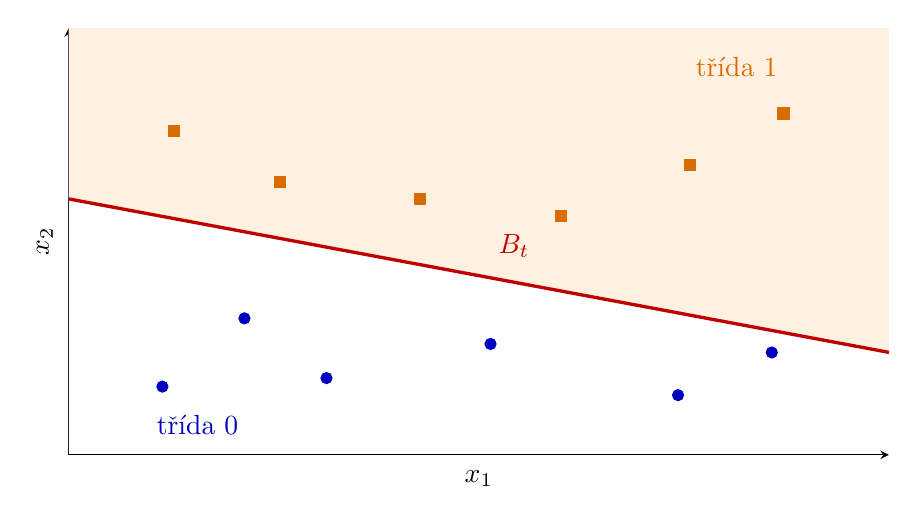
\begin{tikzpicture}
    \begin{axis}[
        width=12cm,height=7cm,
        xmin=0,xmax=7,ymin=0,ymax=5,
        axis lines=left,xlabel={$x_1$},ylabel={$x_2$},
        xtick=\empty,ytick=\empty,
        label style={font=\normalsize},
        every node/.style={font=\normalsize},
        clip=false
    ]
        \addplot[draw=none,fill=orange!12]
        coordinates{(0,3)(7,1.2)(7,5)(0,5)}\closedcycle;
        \addplot[red!75!black,very thick,domain=0:7]{3-0.257*x};
        \addplot[only marks,mark=*,blue!75!black]
        coordinates{(0.8,0.8)(1.5,1.6)(2.2,0.9)(3.6,1.3)(5.2,0.7)(6,1.2)};
        \addplot[only marks,mark=square*,orange!85!black]
        coordinates{(0.9,3.8)(1.8,3.2)(3,3)(4.2,2.8)(5.3,3.4)(6.1,4)};
        \node[red!75!black] at (axis cs:3.8,2.45){\(B_t\)};
        \node[blue!75!black] at (axis cs:1.1,0.35){třída \(0\)};
        \node[orange!85!black] at (axis cs:5.7,4.55){třída \(1\)};
    \end{axis}
\end{tikzpicture}

    \caption{Rozhodovací hranice odděluje oblasti různých předpovědí.}
    \label{fig:ai-rozhodovaci-hranice}
\end{figure}

Cílem není pouze správně klasifikovat trénovací objekty. Model má zachytit vztah mezi znaky a~třídou tak, aby správně pracoval také s~novými objekty. Příliš složitá hranice může obejít každý trénovací bod, ale na neznámých datech selhat.

\section{Logistická regrese}\label{sec:ai-logisticka-regrese}

Při binární klasifikaci používáme třídy \(0\) a~\(1\). Přímé použití lineární regrese je problematické, protože funkce \(ax+b\) může nabývat libovolných reálných hodnot a~čtvercová chyba není přizpůsobena vyhodnocování jistoty klasifikační odpovědi. Logistická regrese proto lineární skóre převádí do intervalu \((0,1)\).

\begin{definition}\label{def:ai-sigmoida}
    \emph{Logistická funkce} neboli \emph{sigmoida} je funkce
    \[
        \sigma(z)
        =
        \frac{1}{1+e^{-z}},
        \qquad z\in\R.
    \]
\end{definition}

Funkce je rostoucí, platí \(\sigma(0)=0{,}5\) a~její hodnoty se pro velmi záporná, respektive velmi kladná \(z\), blíží \(0\), respektive \(1\).

\begin{figure}[ht]
    \centering
    \begin{tikzpicture}
    \begin{axis}[
        width=11cm,height=6cm,
        xmin=-6,xmax=6,ymin=0,ymax=1.05,
        axis lines=middle,xlabel={$z$},ylabel={$\sigma(z)$},
        xtick={0},ytick={0,0.5,1},
        yticklabels={$0$,$0{,}5$,$1$},
        label style={font=\normalsize},
        tick label style={font=\normalsize},
        every node/.style={font=\normalsize},
        clip=false
    ]
        \addplot[blue!75!black,very thick,domain=-6:6,samples=100]
            {1/(1+exp(-x))};
        \addplot[gray,dashed,domain=-6:6]{0.5};
    \end{axis}
\end{tikzpicture}

    \caption{Logistická funkce převádí reálné skóre do intervalu \((0,1)\).}
    \label{fig:ai-sigmoida}
\end{figure}

Pro jeden vstupní statistický soubor
\[
    \mathbf{X}=(x_1,\ldots,x_n)
\]
logistický model nejprve vypočítá lineární skóre \(z_i=ax_i+b\) a~potom
\[
    \hat p_i
    =
    \sigma(z_i)
    =
    \frac{1}{1+e^{-(ax_i+b)}}.
\]
Statistický soubor výstupů označíme
\[
    \hat{\mathbf{P}}
    =
    (\hat p_1,\ldots,\hat p_n).
\]
Hodnotu \(\hat p_i\) chápeme jako míru podpory modelu pro třídu \(1\).

Pro rozhodovací práh \(t\in(0,1)\) definujeme
\[
    h^{(t)}(x)
    =
    \begin{cases}
        1, & \hat p(x)\geqslant t,\\
        0, & \hat p(x)<t.
    \end{cases}
\]
Protože je sigmoida rostoucí,
\[
    \hat p(x)\geqslant t
    \quad\Longleftrightarrow\quad
    ax+b\geqslant
    \ln\left(\frac{t}{1-t}\right).
\]
Pro obvyklý práh \(t=0{,}5\) rozhoduje znaménko výrazu \(ax+b\).

\subsection{Křížová entropie}

\begin{definition}\label{def:ai-bce}
    Pro skutečnou třídu \(y_i\in\set{0,1}\) a~výstup
    \(\hat p_i\in(0,1)\) definujeme \emph{binární křížovou entropii}
    \[
        \ell(y_i,\hat p_i)
        =
        -
        \left(
            y_i\ln\hat p_i
            +(1-y_i)\ln(1-\hat p_i)
        \right).
    \]
    Průměrná křížová entropie na celém souboru je
    \[
        L(\mathbf{Y},\hat{\mathbf{P}})
        =
        \frac1n\sum_{i=1}^{n}\ell(y_i,\hat p_i).
    \]
\end{definition}

Je-li \(y_i=1\), ztráta má tvar \(-\ln\hat p_i\); je-li \(y_i=0\), má tvar \(-\ln(1-\hat p_i)\). Správná a~jistá předpověď má malou ztrátu, zatímco jistá chybná předpověď je potrestána velmi vysokou hodnotou.

Parametry logistické regrese hledáme tak, aby
\[
    (a^\ast,b^\ast)
    =
    \argmin_{(a,b)\in\R^2}L(a,b),
\]
kde
\[
    L(a,b)
    =
    -\frac1n\sum_{i=1}^{n}
    \left(
        y_i\ln\hat p_i(a,b)
        +(1-y_i)\ln(1-\hat p_i(a,b))
    \right).
\]

\subsection{Odbočka: co vyjadřuje derivace}\label{subsec:ai-derivace}

K~hledání minima potřebujeme vědět, jak se hodnota funkce změní při malé změně jejího vstupu. Pro funkci jedné proměnné \(g\) porovnáváme hodnoty \(g(c)\) a~\(g(c+h)\). Podíl
\[
    \frac{g(c+h)-g(c)}{h}
\]
je směrnice sečny vedené dvěma blízkými body grafu. Necháme-li nenulové \(h\) přibližovat k~nule a~směrnice se ustálí, získáme \emph{derivaci} \(g'(c)\). Derivace tedy popisuje okamžitý směr a~rychlost změny:
\begin{itemize}
    \item \(g'(c)>0\): funkce v~okolí \(c\) roste;
    \item \(g'(c)<0\): funkce v~okolí \(c\) klesá;
    \item \(g'(c)=0\): graf má v~daném bodě vodorovnou tečnu; může zde ležet minimum nebo maximum.
\end{itemize}

\begin{figure}[ht]
    \centering
    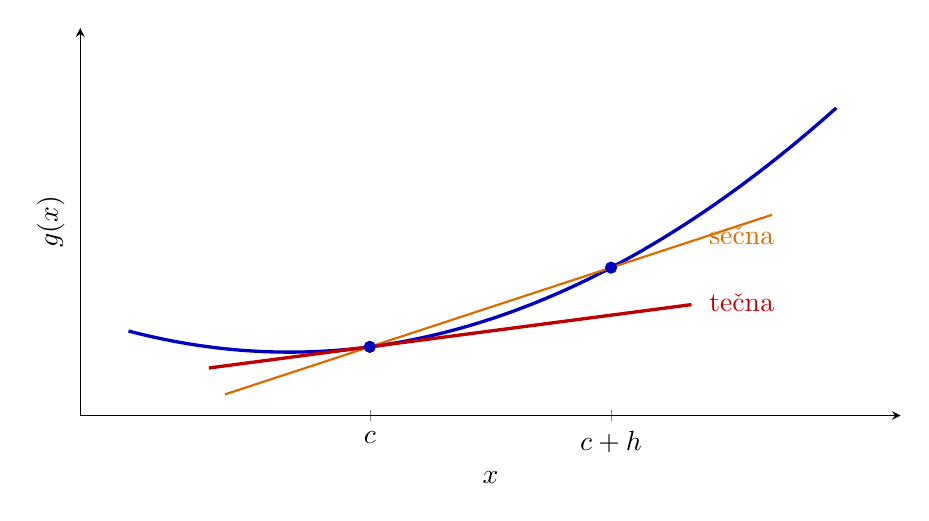
\begin{tikzpicture}
    \begin{axis}[
        width=12cm,height=6.5cm,
        xmin=-0.3,xmax=4.8,ymin=-0.3,ymax=5.2,
        axis lines=left,xlabel={$x$},ylabel={$g(x)$},
        xtick={1.5,3},xticklabels={$c$,$c+h$},
        ytick=\empty,
        label style={font=\normalsize},
        tick label style={font=\normalsize},
        every node/.style={font=\normalsize},
        clip=false
    ]
        \addplot[blue!75!black,very thick,domain=0:4.4,samples=100]
            {0.3*(x-1)^2+0.6};
        % Sečna prochází body (c,g(c))=(1.5,0.675) a
        % (c+h,g(c+h))=(3,1.8); její směrnice je 0.75.
        \addplot[orange!85!black,thick,domain=0.6:4]
            {0.75*x-0.45};
        % Derivace g'(x)=0.6(x-1), takže tečna v c=1.5 má
        % směrnici 0.3 a rovnici y=0.3x+0.225.
        \addplot[red!75!black,very thick,domain=0.5:3.5]
            {0.3*x+0.225};
        \addplot[only marks,mark=*,blue!75!black]
            coordinates{(1.5,0.675)(3,1.8)};
        \node[orange!85!black,anchor=west] at (axis cs:3.55,2.25){sečna};
        \node[red!75!black,anchor=west] at (axis cs:3.55,1.30){tečna};
    \end{axis}
\end{tikzpicture}

    \caption{Sečna se při zmenšování \(h\) blíží tečně; její směrnice je derivací.}
    \label{fig:ai-derivace}
\end{figure}

Závisí-li ztráta \(L(a,b)\) na dvou parametrech, můžeme měnit vždy jen jeden z~nich. Symboly
\[
    \frac{\partial L}{\partial a},
    \qquad
    \frac{\partial L}{\partial b}
\]
označují derivace podle \(a\), respektive podle \(b\), při pevném druhém parametru. Vektor
\[
    \nabla L(a,b)
    =
    \left(
        \frac{\partial L}{\partial a},
        \frac{\partial L}{\partial b}
    \right)
\]
nazýváme \emph{gradient}. Ukazuje směrem nejrychlejšího růstu ztráty, a~proto se při minimalizaci pohybujeme opačným směrem.

\subsection{Gradientní sestup}

Pro logistickou regresi lze odvodit
\[
    \frac{\partial L}{\partial a}
    =
    \frac1n\sum_{i=1}^{n}
    (\hat p_i-y_i)x_i,
    \qquad
    \frac{\partial L}{\partial b}
    =
    \frac1n\sum_{i=1}^{n}
    (\hat p_i-y_i).
\]
Při rychlosti učení \(\eta>0\) opakujeme aktualizace
\[
    a
    \gets
    a-\eta\frac{\partial L}{\partial a},
    \qquad
    b
    \gets
    b-\eta\frac{\partial L}{\partial b}.
\]

\begin{figure}[ht]
    \centering
    \begin{tikzpicture}
    \begin{axis}[
        width=12cm,height=6.2cm,
        xmin=-4,xmax=6,ymin=0,ymax=9,
        axis lines=left,xlabel={parametr},ylabel={\(L\)},
        xtick=\empty,ytick=\empty,
        label style={font=\normalsize},
        every node/.style={font=\normalsize},
        clip=false
    ]
        \addplot[blue!75!black,very thick,domain=-3.8:5.8,samples=100]
            {0.3*(x-1)^2+0.5};
        \foreach \x in {5,3.4,2.3,1.6,1.2}{
            \pgfmathsetmacro{\y}{0.3*(\x-1)^2+0.5}
            \addplot[only marks,mark=*,mark size=2.5pt,red!75!black]
                coordinates{(\x,\y)};
        }
        \draw[diredge,red!75!black] (axis cs:5,5.3)--(axis cs:3.4,2.228);
        \draw[diredge,red!75!black] (axis cs:3.4,2.228)--(axis cs:2.3,1.007);
        \draw[diredge,red!75!black] (axis cs:2.3,1.007)--(axis cs:1.6,0.608);
        \draw[diredge,red!75!black] (axis cs:1.6,0.608)--(axis cs:1.2,0.512);
        \node[above] at (axis cs:1,0.72){minimum};
    \end{axis}
\end{tikzpicture}

    \caption{Gradientní sestup postupně snižuje hodnotu ztrátové funkce.}
    \label{fig:ai-gradientni-sestup}
\end{figure}

Příliš malá \(\eta\) vede k~pomalému postupu. Příliš velká hodnota může minimum přeskakovat nebo výpočet rozkmitat. Zastavujeme například po pevném počtu iterací nebo ve chvíli, kdy se ztráta a~parametry mění už jen nepatrně.

Jedna iterace využije všechny trénovací objekty k~výpočtu průměrného gradientu. Takové variantě říkáme \emph{dávkový gradientní sestup}. U~velkých souborů lze gradient odhadovat z~menších náhodných dávek; aktualizace jsou potom levnější, ale jejich směr více kolísá.

\begin{algorithm}
    \caption{\textsc{logistic-regression}}
    \label{alg:ai-logistic-regression}
    \KwIn{Soubory \(\mathbf{X}=(x_1,\ldots,x_n)\), \(\mathbf{Y}=(y_1,\ldots,y_n)\), rychlost učení \(\eta>0\) a~počet iterací \(T\)}
    \(a\gets0\), \(b\gets0\)\\
    \For{\(r\gets1,2,\ldots,T\)}{
        \For{\(i\gets1,2,\ldots,n\)}{
            \(\displaystyle\hat p_i\gets\frac{1}{1+e^{-(ax_i+b)}}\)
        }
        \(\displaystyle g_a\gets\frac1n\sum_{i=1}^{n}(\hat p_i-y_i)x_i\)\\
        \(\displaystyle g_b\gets\frac1n\sum_{i=1}^{n}(\hat p_i-y_i)\)\\
        \(a\gets a-\eta g_a\), \(b\gets b-\eta g_b\)
    }
    \KwOut{Parametry \(a,b\) a~skóre \(\hat p(x)=\sigma(ax+b)\)}
\end{algorithm}

\subsection{Implementace v~Pythonu}

Program~\ref{lst:ai-logistic-regression} používá přesně uvedené dva gradienty. Metoda \texttt{fit} opakovaně vypočítá všechny hodnoty \(\hat p_i\) a~upraví parametry \(a,b\); metoda \texttt{predict} převede výstupy na třídy pomocí zvoleného prahu.

Funkce \texttt{sigmoid} je zapsána ve dvou algebraicky ekvivalentních větvích. Pro záporné \(z\) používá výraz s~\(e^z\), aby při velmi záporném vstupu nemusela počítat obrovskou hodnotu \(e^{-z}\). Jde o~technickou úpravu numerické stability, nikoli o~změnu matematického modelu.

\lstinputlisting[
    caption={Logistická regrese pro jeden vstupní statistický znak.},
    label={lst:ai-logistic-regression}
]{07-ai/code/logistic_regression.py}

Ukázka používá jeden vstupní znak, aby byl vztah mezi parametry a~rozhodovací hranicí dobře vidět. Pro více znaků nahradíme \(ax+b\) výrazem \(\sum_{j=1}^{p}w_jx_j+\theta\) a~pro každou váhu \(w_j\) počítáme vlastní složku gradientu; princip pseudokódu zůstává stejný.

\section{Vyhodnocení klasifikace}\label{sec:ai-vyhodnoceni-klasifikace}

U~binární klasifikace porovnáváme skutečnou třídu \(y_i\in\set{0,1}\) s~předpovědí \(\hat y_i^{(t)}=h^{(t)}(\mathbf{x}_i)\). Mohou nastat čtyři výsledky:
\begin{itemize}
    \item správně pozitivní: \(y_i=1\) a~\(\hat y_i^{(t)}=1\);
    \item správně negativní: \(y_i=0\) a~\(\hat y_i^{(t)}=0\);
    \item falešně pozitivní: \(y_i=0\), ale \(\hat y_i^{(t)}=1\);
    \item falešně negativní: \(y_i=1\), ale \(\hat y_i^{(t)}=0\).
\end{itemize}

Jejich počty značíme
\[
    \TP_{\mathbf{X},\mathbf{Y}}^{(t)},
    \quad
    \TN_{\mathbf{X},\mathbf{Y}}^{(t)},
    \quad
    \FP_{\mathbf{X},\mathbf{Y}}^{(t)},
    \quad
    \FN_{\mathbf{X},\mathbf{Y}}^{(t)}.
\]
Například
\[
    \TP_{\mathbf{X},\mathbf{Y}}^{(t)}
    =
    \sizeof{
        \set{
            i:y_i=1,\ h^{(t)}(\mathbf{x}_i)=1
        }
    }.
\]
Ostatní tři počty definujeme analogicky. Je-li z~kontextu jasný soubor i~práh, budeme jejich dolní a~horní indexy někdy vynechávat.

\begin{figure}[ht]
    \centering
    \begin{tikzpicture}[every node/.style={font=\normalsize}]
    \node[task,fill=green!12,minimum width=43mm,minimum height=16mm]
        (tp) at (0,0) {\(\TP\)\\správně pozitivní};
    \node[task,fill=red!10,minimum width=43mm,minimum height=16mm]
        (fn) at (4.7,0) {\(\FN\)\\falešně negativní};
    \node[task,fill=red!10,minimum width=43mm,minimum height=16mm]
        (fp) at (0,-2) {\(\FP\)\\falešně pozitivní};
    \node[task,fill=green!12,minimum width=43mm,minimum height=16mm]
        (tn) at (4.7,-2) {\(\TN\)\\správně negativní};
    \node[above=7mm of tp] {předpověď \(1\)};
    \node[above=7mm of fn] {předpověď \(0\)};
    \node[left=5mm of tp,align=right] {skutečnost\\\(1\)};
    \node[left=5mm of fp,align=right] {skutečnost\\\(0\)};
\end{tikzpicture}

    \caption{Matice záměn pro binární klasifikaci.}
    \label{fig:ai-matice-zamen}
\end{figure}

\subsection{Správnost, přesnost, pokrytí a~\(F_1\)-míra}

\begin{definition}\label{def:ai-klasifikacni-metriky}
    Jsou-li příslušné jmenovatele nenulové, definujeme
    \begin{align*}
        \Accuracy_{\mathbf{X},\mathbf{Y}}^{(t)}
        &=
        \frac{\TP+\TN}{\TP+\TN+\FP+\FN},\\
        \Precision_{\mathbf{X},\mathbf{Y}}^{(t)}
        &=
        \frac{\TP}{\TP+\FP},\\
        \Recall_{\mathbf{X},\mathbf{Y}}^{(t)}
        &=
        \frac{\TP}{\TP+\FN},\\
        \Fscore_{1,\mathbf{X},\mathbf{Y}}^{(t)}
        &=
        \frac{2}{
            (\Precision_{\mathbf{X},\mathbf{Y}}^{(t)})^{-1}
            +
            (\Recall_{\mathbf{X},\mathbf{Y}}^{(t)})^{-1}
        }.
    \end{align*}
\end{definition}

\emph{Správnost} (anglicky \emph{accuracy}) odpovídá podílu všech správných odpovědí. \emph{Přesnost} (anglicky \emph{precision}) se ptá, kolika pozitivním předpovědím můžeme věřit. \emph{Pokrytí} (anglicky \emph{recall}) se ptá, jakou část skutečně pozitivních objektů jsme nalezli. \(F_1\)-míra je harmonický průměr přesnosti a~pokrytí a~je vysoká pouze tehdy, jsou-li vysoké obě hodnoty.

Dosazením definic dostaneme užitečný tvar
\[
    \Fscore_{1,\mathbf{X},\mathbf{Y}}^{(t)}
    =
    \frac{2\TP}{2\TP+\FP+\FN}.
\]

\begin{example}
    Pro
    \[
        \TP=36,\qquad
        \TN=44,\qquad
        \FP=8,\qquad
        \FN=12
    \]
    vychází
    \[
        \Accuracy=0{,}80,
        \quad
        \Precision\doteq0{,}82,
        \quad
        \Recall=0{,}75,
        \quad
        \Fscore_1\doteq0{,}78.
    \]
\end{example}

Správnost může být zavádějící u~nevyvážených tříd. Jestliže je mezi tisícem zpráv pouze deset podvodných, klasifikátor označující vždy běžnou zprávu dosáhne správnosti \(0{,}99\), ale jeho pokrytí podvodných zpráv je nulové.

\subsection{Vliv prahu a~neznámá data}

Snížení rozhodovacího prahu obvykle zvýší počet pozitivních předpovědí. Tím může růst pokrytí, ale zároveň přibývají falešně pozitivní výsledky a~klesá přesnost. Vhodný práh proto volíme podle důsledků obou typů chyb a~podle výsledků na validačních datech.

V~lékařském předběžném vyšetření může být závažnější přehlédnout nemocného člověka než poslat zdravého na další kontrolu; dává proto smysl upřednostnit vysoké pokrytí. U~automatického blokování účtů může být naopak falešně pozitivní rozhodnutí velmi nákladné, a~proto požadujeme vysokou přesnost. Jediná metrika bez kontextu tyto rozdíly nezachytí.

Změnou prahu získáme celou rodinu klasifikátorů ze stejného skórovacího modelu. Při jejich porovnávání sledujeme, jak se současně mění podíl správně pozitivních a~falešně pozitivních odpovědí. Tím lze hodnotit kvalitu samotného pořadí objektů podle skóre odděleně od volby jednoho konkrétního prahu.

\warningbox{Metriky uváděné po dokončení vývoje modelu počítáme na testovacích datech, která nebyla použita ani k~trénování, ani k~volbě prahu či jiných nastavení. Jinak získáme příliš optimistický odhad kvality.}

\section{Algoritmus \(k\)-NN}\label{sec:ai-knn}

Metoda \(k\) nejbližších sousedů (anglicky \emph{\(k\)-nearest neighbors}, \(k\)-NN) vychází z~intuice, že podobné objekty mívají stejnou třídu. Nevytváří předem parametrický vzorec. Při klasifikaci nového objektu přímo vyhledá nejbližší trénovací objekty a~nechá je hlasovat.

\begin{definition}\label{def:ai-eukleidovska-vzdalenost}
    Pro vektory
    \[
        \mathbf{u}=(u_1,\ldots,u_p),
        \qquad
        \mathbf{v}=(v_1,\ldots,v_p)
    \]
    definujeme \emph{eukleidovskou vzdálenost}
    \[
        d_E(\mathbf{u},\mathbf{v})
        =
        \sqrt{
            \sum_{j=1}^{p}(u_j-v_j)^2
        }.
    \]
\end{definition}

Obecně budeme vzdálenost značit \(d(\mathbf{u},\mathbf{v})\). Seřaďme indexy trénovacích objektů tak, aby
\[
    d(\mathbf{x},\mathbf{x}_{\pi(1)})
    \leqslant
    \cdots
    \leqslant
    d(\mathbf{x},\mathbf{x}_{\pi(n)}).
\]
Množina indexů \(k\) nejbližších sousedů je
\[
    N_k(\mathbf{x})
    =
    \set{\pi(1),\ldots,\pi(k)}.
\]

\begin{definition}\label{def:ai-knn}
    Klasifikátor \(k\)-NN je funkce
    \[
        h^{(k)}(\mathbf{x})
        =
        \argmax_{c\in\mathcal{Y}}
        \sizeof{
            \set{
                i\in N_k(\mathbf{x}):y_i=c
            }
        }.
    \]
\end{definition}

\begin{figure}[ht]
    \centering
    \begin{tikzpicture}
    \begin{axis}[
        width=10cm,height=8cm,
        xmin=0,xmax=8,ymin=0,ymax=6,
        axis lines=left,xlabel={$x_1$},ylabel={$x_2$},
        xtick=\empty,ytick=\empty,
        label style={font=\normalsize},
        every node/.style={font=\normalsize},
        clip=false
    ]
        \addplot[only marks,mark=*,mark size=2.5pt,blue!75!black]
            coordinates{(1,1)(1.8,2)(2.7,1.4)(3.4,2.4)(4,1.7)};
        \addplot[only marks,mark=square*,mark size=2.7pt,orange!85!black]
            coordinates{(4.8,3.3)(5.5,2.8)(5.8,4.2)(6.7,3.5)(7.2,4.8)(6.1,1.9)};
        \addplot[only marks,mark=diamond*,mark size=4pt,red!75!black]
            coordinates{(4.6,2.5)};
        \addplot[only marks,mark=o,mark size=6pt,black]
            coordinates{(4,1.7)(3.4,2.4)(4.8,3.3)(5.5,2.8)(6.1,1.9)};
        \draw[dashed,gray] (axis cs:4.6,2.5)--(axis cs:4,1.7);
        \draw[dashed,gray] (axis cs:4.6,2.5)--(axis cs:3.4,2.4);
        \draw[dashed,gray] (axis cs:4.6,2.5)--(axis cs:4.8,3.3);
        \draw[dashed,gray] (axis cs:4.6,2.5)--(axis cs:5.5,2.8);
        \draw[dashed,gray] (axis cs:4.6,2.5)--(axis cs:6.1,1.9);
        \node[red!75!black,anchor=west] at (axis cs:4.75,2.35){\(\mathbf{x}\)};
    \end{axis}
\end{tikzpicture}

    \caption{Klasifikace nového objektu podle pěti nejbližších sousedů.}
    \label{fig:ai-knn}
\end{figure}

Při shodě hlasů potřebujeme předem stanovené pravidlo. U~binární klasifikace se proto často volí liché \(k\). Malé \(k\) vytváří pružnou hranici citlivou na jednotlivé body a~šum. Velké \(k\) rozhodování vyhlazuje, ale může přehlédnout malé místní skupiny. Hodnotu \(k\) proto volíme podle výsledku na validační množině.

Vedle eukleidovské vzdálenosti lze použít například Minkowského vzdálenost
\[
    d_q(\mathbf{u},\mathbf{v})
    =
    \left(
        \sum_{j=1}^{p}
        \abs{u_j-v_j}^q
    \right)^{1/q},
    \qquad q\geqslant1.
\]
Pro \(q=1\) jde o~manhattanskou vzdálenost, pro \(q=2\) o~eukleidovskou. Smysl výsledku vždy závisí na tom, zda zvolená vzdálenost skutečně vystihuje podobnost objektů dané úlohy.

\importantbox{Před použitím \(k\)-NN je obvykle nutné standardizovat nebo normalizovat jednotlivé vstupní znaky. Jinak může znak s~větším číselným měřítkem zcela ovládnout výpočet vzdálenosti.}

\subsection{Implementace v~Pythonu}

Program~\ref{lst:ai-knn} uchovává trénovací objekty a~jejich třídy. Při predikci spočítá všechny vzdálenosti, vybere \(k\) nejmenších a~vrátí nejčastější třídu. V~případě shody rozhodne menší hodnota třídy, aby byl výsledek jednoznačný.

\lstinputlisting[
    caption={Klasifikátor \(k\)-NN s~eukleidovskou vzdáleností.},
    label={lst:ai-knn}
]{07-ai/code/knn.py}

Trénování je téměř okamžité, ale klasifikace nového objektu vyžaduje porovnání s~celou trénovací množinou. Metoda proto přesouvá většinu výpočetní práce do okamžiku použití modelu.

\section{Algoritmus SVM}\label{sec:ai-svm}

Metoda podpůrných vektorů (anglicky \emph{support vector machine}, SVM) hledá rozhodovací hranici, která nejen oddělí třídy, ale ponechá mezi nimi co nejširší volný prostor. Nejprve budeme uvažovat lineárně oddělitelná data.

\subsection{Oddělující nadrovina a~maximální okraj}

Pro nový vektor parametrů
\[
    \mathbf{w}=(w_1,\ldots,w_p)\in\R^p
\]
a~\(\theta\in\R\) zavedeme lineární skóre
\[
    g(\mathbf{x})
    =
    \sum_{j=1}^{p}w_jx_j+\theta.
\]
Rozhodovací hranici tvoří nadrovina
\[
    g(\mathbf{x})=0.
\]
V~rovině jde o~přímku, ve třech rozměrech o~rovinu. Klasifikátor přiřadí třídu \(1\) bodům s~\(g(\mathbf{x})\geqslant0\) a~třídu \(0\) bodům s~\(g(\mathbf{x})<0\).

Vzdálenost bodu \(\mathbf{x}\) od této nadroviny je
\[
    \frac{\abs{g(\mathbf{x})}}{\norm{\mathbf{w}}},
    \qquad
    \norm{\mathbf{w}}
    =
    \sqrt{\sum_{j=1}^{p}w_j^2}.
\]
Samotných oddělujících nadrovin může existovat mnoho. SVM volí takovou, jejíž nejbližší body z~obou tříd jsou od hranice co nejdále. Tento nejmenší odstup nazýváme \emph{okraj} (anglicky \emph{margin}).

\begin{figure}[ht]
    \centering
    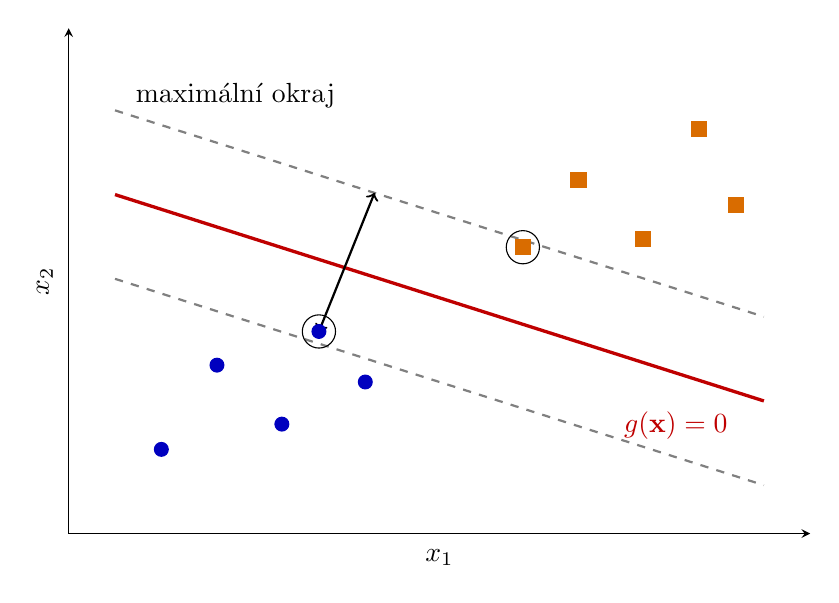
\begin{tikzpicture}
    \begin{axis}[
        width=11cm,height=8cm,
        xmin=0,xmax=8,ymin=0,ymax=6,
        axis lines=left,xlabel={$x_1$},ylabel={$x_2$},
        xtick=\empty,ytick=\empty,
        label style={font=\normalsize},
        every node/.style={font=\normalsize},
        clip=false
    ]
        \addplot[only marks,mark=*,mark size=2.5pt,blue!75!black]
            coordinates{(1,1)(1.6,2)(2.3,1.3)(2.7,2.4)(3.2,1.8)};
        \addplot[only marks,mark=square*,mark size=2.7pt,orange!85!black]
            coordinates{(4.9,3.4)(5.5,4.2)(6.2,3.5)(6.8,4.8)(7.2,3.9)};
        \addplot[red!75!black,very thick,domain=0.5:7.5]{-0.35*x+4.2};
        \addplot[gray,dashed,thick,domain=0.5:7.5]{-0.35*x+3.2};
        \addplot[gray,dashed,thick,domain=0.5:7.5]{-0.35*x+5.2};
        \addplot[only marks,mark=o,mark size=6pt,black]
            coordinates{(2.7,2.4)(4.9,3.4)};
        \node[red!75!black] at (axis cs:6.55,1.28){\(g(\mathbf{x})=0\)};
        \node at (axis cs:1.8,5.2){maximální okraj};
        \draw[<->,thick] (axis cs:2.7,2.4)--(axis cs:3.3,4.045);
    \end{axis}
\end{tikzpicture}

    \caption{Oddělující přímka, maximální okraj a~podpůrné vektory.}
    \label{fig:ai-svm}
\end{figure}

Po vhodném přenásobení \(\mathbf{w}\) a~\(\theta\) můžeme hraniční přímky okraje zapsat
\[
    g(\mathbf{x})=1
    \qquad\text{a}\qquad
    g(\mathbf{x})=-1.
\]
Jejich vzájemná vzdálenost je
\[
    \frac{2}{\norm{\mathbf{w}}}.
\]
Body ležící na hranicích okraje nazýváme \emph{podpůrné vektory}. Právě ony polohu optimální hranice přímo určují. Posun bodu ležícího daleko od okraje ji obvykle nezmění, zatímco posun podpůrného vektoru ano.

Šířku okraje nemůžeme zvětšovat libovolným přenásobením parametrů, protože současně požadujeme, aby trénovací objekty ležely na správné straně hraničních nadrovin. Označíme-li třídy hodnotami \(\tilde y_i=2y_i-1\in\set{-1,1}\), tvrdý okraj splňuje podmínky
\[
    \tilde y_i g(\mathbf{x}_i)\geqslant1
    \qquad\text{pro všechna }i.
\]
Maximalizace šířky \(2/\norm{\mathbf{w}}\) je za těchto podmínek ekvivalentní minimalizaci \(\frac12\norm{\mathbf{w}}^2\).

\subsection{Neoddělitelná data a~měkký okraj}

Reálná data často nelze bez chyby oddělit jedinou nadrovinou. SVM proto může použít \emph{měkký okraj}: připustí některé body uvnitř okraje nebo dokonce na chybné straně hranice. Nastavení modelu pak představuje kompromis mezi dvěma cíli:
\begin{itemize}
    \item mít okraj co nejširší;
    \item mít co nejméně závažných porušení a~chybných klasifikací.
\end{itemize}
Parametr \(C>0\) určuje cenu porušení. Velké \(C\) chyby silně trestá a~obvykle vede k~užšímu okraji. Menší \(C\) dovolí více porušení, ale může vytvořit stabilnější širší hranici. Hodnotu \(C\) volíme pomocí validačních dat.

Míru porušení pro objekt \(i\) lze vyjádřit \emph{pantovou ztrátou} (anglicky \emph{hinge loss})
\[
    \ell_i
    =
    \max\set{0,1-\tilde y_i g(\mathbf{x}_i)}.
\]
Je-li objekt správně za okrajem, platí \(\ell_i=0\). Bod uvnitř okraje má kladnou ztrátu, a~bod na chybné straně rozhodovací hranice ztrátu větší než \(1\). Trénování měkkého okraje lze proto zapsat jako minimalizaci
\[
    \frac12\norm{\mathbf{w}}^2
    +
    C\sum_{i=1}^{n}\ell_i.
\]

Lineární hranice nemusí stačit ani po povolení chyb. Jednou možností je převést objekty do prostoru s~dalšími znaky, v~němž je lze oddělit nadrovinou. Jádrový trik (anglicky \emph{kernel trick}) umožňuje některé takové výpočty provést bez explicitního vytváření všech nových souřadnic. Výsledná hranice v~původním prostoru pak může být nelineární.

Jádro musí vhodným způsobem vyjadřovat podobnost dvojice objektů. Volba lineárního jádra ponechá původní nadrovinu, polynomiální nebo gaussovské jádro umožní zakřivené hranice. Složitější hranice však nemusí lépe zobecňovat, a~proto typ jádra i~jeho parametry volíme podle validačních dat.

\subsection{Vlastnosti a~použití}

Mezi výhody SVM patří jasná geometrická interpretace, možnost nelineárních hranic a~skutečnost, že hranici přímo určuje jen část trénovacích objektů. Metoda může dobře fungovat i~při větším počtu znaků.

Nevýhodou je citlivost na měřítko dat a~na volbu \(C\) a~jádra. U~velkých datových souborů může být trénování náročné a~výstup modelu nemá bez další úpravy přímou pravděpodobnostní interpretaci jako výstup logistické regrese. Typicky se SVM používá pro klasifikaci textu, obrazových znaků nebo biologických dat, zejména není-li počet trénovacích objektů extrémně velký.

Podpůrné vektory zároveň poskytují užitečnou kontrolu modelu. Pokud se jejich malá změna výrazně projeví na rozhodovací hranici, může být model citlivý na šum nebo odlehlá pozorování. Velký počet podpůrných vektorů zase naznačuje, že třídy nejsou zvolenými znaky dobře oddělené.

\warningbox{Stejně jako u~\(k\)-NN je před trénováním SVM obvykle nutné standardizovat nebo normalizovat vstupní znaky. Jinak geometrický okraj odráží především rozdílné jednotky a~měřítko.}

\begin{remark}
    Základy metody podpůrných vektorů vznikaly v~pracích Vladimira Vapnika a~Alexeje Červoněnkise už v~60.~letech 20.~století. Dnes běžnou variantu s~měkkým okrajem popsali Corinna Cortesová a~Vladimir Vapnik roku 1995.
\end{remark}

\subsection{Pseudokód a~implementace}

Pro názornou implementaci použijeme lineární SVM a~stochastický podgradientní sestup. Místo parametru \(C\) budeme regulaci zapisovat pomocí nového parametru \(\lambda>0\) v~ekvivalentně škálovaném cíli
\[
    \frac{\lambda}{2}\norm{\mathbf{w}}^2
    +
    \frac1n\sum_{i=1}^{n}
    \max\set{0,1-\tilde y_i g(\mathbf{x}_i)}.
\]
Větší \(\lambda\) silněji zmenšuje váhy a~upřednostňuje širší okraj; jeho role je tedy opačná než role \(C\).

V~každém kroku nejprve váhy mírně zmenšíme kvůli členu \(\frac{\lambda}{2}\norm{\mathbf{w}}^2\). Pokud vybraný objekt porušuje okraj, přidáme navíc opravu ve směru \(\tilde y_i\mathbf{x}_i\) a~upravíme práh. Jde o~zjednodušený výukový postup; plnohodnotné knihovny používají rychlejší optimalizační metody a~pečlivější volbu rychlosti učení.

\begin{algorithm}
    \caption{\textsc{svm-sgd}}
    \label{alg:ai-svm}
    \KwIn{Trénovací množina \(D\), rychlost učení \(\eta>0\), regulace \(\lambda>0\) a~počet epoch \(T\)}
    \(\mathbf{w}\gets\mathbf{0}\), \(\theta\gets0\)\\
    \For{\(e\gets1,2,\ldots,T\)}{
        \ForEach{\textup{objekt \((\mathbf{x}_i,y_i)\in D\)}}{
            \(\tilde y_i\gets2y_i-1\)\\
            \(\mathbf{w}\gets(1-\eta\lambda)\mathbf{w}\)\\
            \If{\(\tilde y_i(\sum_{j=1}^{p}w_jx_{ij}+\theta)<1\)}{
                \(\mathbf{w}\gets\mathbf{w}+\eta\tilde y_i\mathbf{x}_i\)\\
                \(\theta\gets\theta+\eta\tilde y_i\)
            }
        }
    }
    \KwOut{Klasifikátor \(h(\mathbf{x})=1\), pokud \(\sum_{j=1}^{p}w_jx_j+\theta\geqslant0\), jinak \(0\)}
\end{algorithm}

Program~\ref{lst:ai-svm} odpovídá tomuto pseudokódu. Metoda \texttt{decision\_function} vrací podepsané skóre: jeho znaménko určuje třídu a~jeho absolutní hodnota vyjadřuje vzdálenost od hranice pouze po vydělení normou vah. Metoda \texttt{predict} proto ke klasifikaci používá jen znaménko.

\lstinputlisting[
    caption={Lineární SVM trénované stochastickým podgradientním sestupem.},
    label={lst:ai-svm}
]{07-ai/code/svm.py}

Příklad obsahuje dvě lineárně oddělitelné skupiny bodů. Po natrénování program vypíše parametry hranice a~třídy několika nových objektů. Před použitím na reálných datech bychom vstupní znaky standardizovali a~hodnoty \(\lambda\), \(\eta\) i~počet epoch zvolili podle validační množiny.

\section{Úvod do neuronových sítí}\label{sec:ai-uvod-neuronove-site}

Lineární a~logistická regrese skládají výstup z~jediného lineárního skóre. Takový model vytváří lineární rozhodovací hranici a~nemůže sám zachytit složitější vztahy. Neuronová síť spojuje větší počet jednoduchých výpočetních jednotek do vrstev. Výstup jedné vrstvy se stává vstupem vrstvy následující, takže síť může postupně vytvářet stále složitější reprezentace dat.

Název vznikl volnou inspirací biologickými neurony. Biologický neuron přijímá signály dendrity, zpracovává je v~těle buňky a~při dostatečném podráždění vysílá signál axonem. Formální neuron tento proces výrazně zjednodušuje: vstupy vynásobí vahami, sečte je, přidá práh a~na výsledek použije aktivační funkci.

\begin{figure}[ht]
    \centering
    \begin{tikzpicture}[
    neuron/.style={circle, draw=darkblue, very thick, fill=darkblue!10, minimum size=14mm},
    box/.style={draw=darkblue, rounded corners, fill=darkblue!8, minimum width=23mm, minimum height=11mm, align=center},
    conn/.style={-Latex, very thick, draw=darkblue}
]
    \node[neuron] (body) at (0,0) {tělo};
    \foreach \ang in {120,150,180,210,240}
        \draw[very thick, darkblue] (body) -- ++(\ang:13mm) -- ++(\ang+15:6mm);
    \draw[conn] (body) -- node[above] {axon} ++(2.3,0);
    \node[above=7mm of body] {biologický neuron};

    \node[box] (sum) at (5.2,0) {vážený\\součet};
    \node[box, right=15mm of sum] (act) {aktivační\\funkce \(f\)};
    \draw[conn] ([xshift=-14mm]sum.west) -- node[above] {vstupy} (sum.west);
    \draw[conn] (sum) -- (act);
    \draw[conn] (act.east) -- ++(14mm,0) node[right] {výstup};
    \node[above=7mm of $(sum)!0.5!(act)$] {formální neuron};

    \draw[conn, dashed] (2.2,-1.4) -- node[below] {zjednodušení} (4.5,-1.4);
\end{tikzpicture}


    \caption{Biologická inspirace a~její zjednodušení na formální neuron.}
    \label{fig:ai-biologicky-formalni}
\end{figure}

\warningbox{Neuronová síť není přesným modelem lidského mozku. Podobnost spočívá především v~propojení mnoha jednoduchých jednotek. Způsob výpočtu i~učení běžných sítí je matematickou konstrukcí navrženou pro zpracování dat.}

Váha spoje určuje, jak silně daný vstup ovlivní výsledek. Kladná váha vliv podporuje, záporná jej potlačuje a~váha blízká nule jej téměř ignoruje. Učení sítě spočívá v~hledání takových vah a~prahů, při nichž budou její výstupy na trénovacích datech co nejméně chybné.

Neuronové sítě se používají například pro rozpoznávání obrazu a~řeči, zpracování textu, předpovídání časových řad nebo řízení. Jejich výhodou je schopnost modelovat složité nelineární vztahy. Cenou za tuto obecnost je větší množství dat a~výpočtů potřebných k~učení a~také obtížnější vysvětlitelnost výsledku.

\begin{remark}
    Frank Rosenblatt představil perceptron roku 1957 a~první hardwarovou realizaci Mark~I Perceptron dokončil roku 1958. Zpětné šíření chyby bylo známé v~různých podobách dříve, ale jeho význam pro učení vícevrstvých sítí výrazně zpopularizovala práce Davida Rumelharta, Geoffreyho Hintona a~Ronalda Williamse z~roku 1986.
\end{remark}

\section{Formální neuronová síť}\label{sec:ai-formalni-neuronova-sit}

\subsection{Formální neuron}

Uvažujme objekt \(\mathbf{x}_i=(x_{i1},\ldots,x_{ip})\in\R^p\). Formální neuron má pro každý vstup váhu \(w_j\in\R\), práh \(\theta\in\R\) a~aktivační funkci \(f\). Nejprve vypočítá lineární kombinaci
\[
    z_i
    =
    \sum_{j=1}^{p}w_jx_{ij}+\theta
\]
a~potom výstup
\[
    \hat y_i=f(z_i).
\]
Práh \(\theta\) lze chápat jako váhu dodatečného stálého vstupu \(1\). V~některých zdrojích se proto nazývá posunutí (anglicky \emph{bias}).

\begin{figure}[ht]
    \centering
    \begin{tikzpicture}[
    input/.style={circle, draw=darkblue, fill=darkblue!8, minimum size=9mm},
    block/.style={circle, draw=darkblue, very thick, fill=darkblue!12, minimum size=18mm, align=center},
    conn/.style={-Latex, thick, draw=darkblue}
]
    \node[input] (x1) at (0,1.8) {\(x_{i1}\)};
    \node[input] (x2) at (0,0.6) {\(x_{i2}\)};
    \node at (0,-0.3) {\(\vdots\)};
    \node[input] (xp) at (0,-1.3) {\(x_{ip}\)};
    \node[block] (sum) at (3.2,0.3) {\(\sum\)};
    \node[block] (act) at (6.0,0.3) {\(f\)};

    \draw[conn] (x1) -- node[above, sloped] {\(w_1\)} (sum);
    \draw[conn] (x2) -- node[above, sloped] {\(w_2\)} (sum);
    \draw[conn] (xp) -- node[below, sloped] {\(w_p\)} (sum);
    \draw[conn] ([yshift=-18mm]sum.south) -- node[right] {\(\theta\)} (sum.south);
    \draw[conn] (sum) -- node[above] {\(z_i\)} (act);
    \draw[conn] (act.east) -- ++(15mm,0) node[right] {\(\hat y_i\)};
\end{tikzpicture}


    \caption{Formální neuron: vážený součet vstupů následovaný aktivační funkcí.}
    \label{fig:ai-formalni-neuron}
\end{figure}

Volbou schodové aktivační funkce
\[
    f(z)
    =
    \begin{cases}
        1, & z\geqslant0,\\
        0, & z<0
    \end{cases}
\]
získáme \emph{perceptron}. Jeho rozhodovací hranice
\[
    \sum_{j=1}^{p}w_jx_j+\theta=0
\]
je nadrovina. Jeden perceptron tedy dokáže oddělit pouze lineárně oddělitelné třídy.

V~hlubších sítích potřebujeme aktivační funkce, které dovolují postupně upravovat váhy pomocí derivací. Často používáme sigmoidální funkci zavedenou v~\smartref[definici~][]{\showrefs}{def:ai-sigmoida}{definici sigmoidy} nebo funkci
\[
    \ReLU(z)=\max\set{0,z}.
\]
Funkce \(\ReLU\) ponechá kladný vstup beze změny a~záporný nahradí nulou. Pro rozdělení výstupu mezi \(k\) tříd se používá funkce \emph{softmax}. Pro vektor skóre
\(\mathbf{z}=(z_1,\ldots,z_k)\in\R^k\) vrací
\[
    \sigma_i(\mathbf{z})
    =
    \frac{e^{z_i}}{\sum_{j=1}^{k}e^{z_j}},
    \qquad i\in\set{1,\ldots,k}.
\]
Všechny hodnoty \(\sigma_i(\mathbf{z})\) jsou kladné a~jejich součet je \(1\).

\subsection{Síť a~vrstvy}

\begin{definition}\label{def:ai-formalni-sit}
    \emph{Formální neuronová síť} je uspořádaná sedmice
    \[
        \mathcal N=(V,E,I,O,w,\theta,f),
    \]
    kde \(V\) je konečná množina neuronů, \(E\subseteq V\times V\) je množina orientovaných spojů, \(I\subseteq V\) je množina vstupních neuronů, \(O\subseteq V\) je množina výstupních neuronů, \(w\colon E\to\R\) přiřazuje spojům váhy, \(\theta\colon V\setminus I\to\R\) přiřazuje nevstupním neuronům prahy a~\(f\colon\R\to\R\) je aktivační funkce.
\end{definition}

Je-li graf \((V,E)\) acyklický a~spoje vedou pouze od dřívější vrstvy k~pozdější, hovoříme o~\emph{dopředné neuronové síti}. Neurony rozdělíme do vstupní vrstvy, jedné nebo více skrytých vrstev a~výstupní vrstvy.

\begin{figure}[ht]
    \centering
    \begin{tikzpicture}[
    neuron/.style={circle, draw=darkblue, fill=darkblue!9, minimum size=8mm},
    conn/.style={draw=darkblue!65, thin}
]
    \foreach \y/\name in {1.6/x1,0/x2,-1.6/xp}
        \node[neuron] (\name) at (0,\y) {};
    \node at (0,-0.75) {\(\vdots\)};
    \node[left=3mm of x1] {\(x_{i1}\)};
    \node[left=3mm of x2] {\(x_{i2}\)};
    \node[left=3mm of xp] {\(x_{ip}\)};

    \foreach \y/\name in {2.0/h1,0.7/h2,-0.7/h3,-2.0/h4}
        \node[neuron] (\name) at (3.1,\y) {};

    \foreach \y/\name in {0.8/o1,-0.8/o2}
        \node[neuron] (\name) at (6.2,\y) {};

    \foreach \a in {x1,x2,xp}
        \foreach \b in {h1,h2,h3,h4}
            \draw[conn] (\a) -- (\b);
    \foreach \a in {h1,h2,h3,h4}
        \foreach \b in {o1,o2}
            \draw[conn] (\a) -- (\b);

    \node[above=4mm of x1] {vstupní vrstva};
    \node[above=4mm of h1] {skrytá vrstva};
    \node[above=4mm of o1] {výstupní vrstva};
    \node[right=3mm of o1] {\(\hat y_{i1}\)};
    \node[right=3mm of o2] {\(\hat y_{i2}\)};
\end{tikzpicture}


    \caption{Vícevrstvý perceptron se vstupní, skrytou a~výstupní vrstvou.}
    \label{fig:ai-mlp}
\end{figure}

Počet skrytých vrstev označíme \(L-1\). Aktivace vstupní vrstvy pro objekt \(\mathbf{x}_i\) tvoří vektor
\[
    \mathbf{a}^{(0)}=\mathbf{x}_i.
\]
Má-li vrstva \(\ell\) celkem \(n_\ell\) neuronů, označíme její aktivace
\[
    \mathbf{a}^{(\ell)}
    =
    \left(
        a_1^{(\ell)},\ldots,a_{n_\ell}^{(\ell)}
    \right).
\]
Váhu spoje z~\(j\)-tého neuronu vrstvy \(\ell\) do \(r\)-tého neuronu vrstvy \(\ell+1\) označíme
\[
    w_{jr}^{(\ell+1)}
\]
a~práh cílového neuronu \(\theta_r^{(\ell+1)}\). Přenosovou funkci této vrstvy označíme \(f^{(\ell+1)}\). Potom
\[
    a_r^{(\ell+1)}
    =
    f^{(\ell+1)}\left(
        \sum_{j=1}^{n_\ell}
        w_{jr}^{(\ell+1)}a_j^{(\ell)}
        +
        \theta_r^{(\ell+1)}
    \right).
\]
Výpočet opakujeme od \(\ell=0\) až k~výstupní vrstvě \(L\). Tento postup nazýváme \emph{dopředný průchod}.

\tipbox{Kdyby ve všech vrstvách byla aktivační funkce \(f(z)=z\), celá síť by byla pouze složením lineárních funkcí, a~tedy opět jedinou lineární funkcí. Nelineární aktivační funkce jsou proto nezbytné pro modelování složitějších hranic.}

\section{Učení neuronové sítě}\label{sec:ai-uceni-neuronove-site}

Při učení s~učitelem máme trénovací data
\[
    D
    =
    \set{
        (\mathbf{x}_1,y_1),\ldots,(\mathbf{x}_n,y_n)
    }.
\]
Síť pro každý vstup provede dopředný průchod a~vytvoří výstup \(\hat y_i\). Ztrátová funkce porovná \(\hat y_i\) se správnou hodnotou \(y_i\). Pro regresi může jít o~MSE, pro binární klasifikaci o~křížovou entropii. Cílem je upravit všechny váhy a~prahy tak, aby byla průměrná ztráta co nejmenší.

\subsection{Zpětné šíření chyby}

Derivaci jsme v~\smartref[podsekci~][]{\showrefs}{subsec:ai-derivace}{předchozím výkladu} popsali jako citlivost výstupu na malou změnu vstupu. Ve vícevrstvé síti potřebujeme určit citlivost ztráty na každou váhu. Změna váhy v~první vrstvě nejprve změní aktivaci příslušného neuronu, ta ovlivní další vrstvu a~teprve nakonec výstup a~ztrátu.

Algoritmus \emph{zpětného šíření chyby} (anglicky \emph{backpropagation}) tyto závislosti počítá odzadu. Nejprve určí, jak změna výstupu ovlivní ztrátu. Potom postupuje od výstupní vrstvy ke vstupní a~pro každý spoj násobí lokální citlivosti na navazující části výpočtu. Tím získá derivaci ztráty podle každé váhy a~prahu.

\begin{figure}[ht]
    \centering
    \begin{tikzpicture}[
    block/.style={draw=darkblue, rounded corners, fill=darkblue!8, minimum width=23mm, minimum height=11mm, align=center},
    fwd/.style={-Latex, very thick, draw=darkblue},
    back/.style={-Latex, very thick, dashed, draw=red!75!black}
]
    \node[block] (input) at (0,0) {vstup\\\(\mathbf{x}_i\)};
    \node[block] (hidden) at (3.0,0) {skrytá\\vrstva};
    \node[block] (output) at (6.0,0) {výstup\\\(\hat y_i\)};
    \node[block] (loss) at (9.0,0) {chyba\\\(E_i\)};

    \draw[fwd] (input) -- node[above] {aktivace} (hidden);
    \draw[fwd] (hidden) -- node[above] {aktivace} (output);
    \draw[fwd] (output) -- (loss);

    \draw[back] ([yshift=-3mm]loss.south west) to[bend left=18]
        node[below] {gradienty} ([yshift=-3mm]hidden.south east);
    \draw[back] ([yshift=-3mm]hidden.south west) to[bend left=18]
        ([yshift=-3mm]input.south east);
\end{tikzpicture}

    \caption{Dopředný průchod počítá výstup; zpětný průchod přenáší informaci o~chybě.}
    \label{fig:ai-backprop}
\end{figure}

Například pro jediný neuron
\[
    z=\sum_{j=1}^{p}w_jx_j+\theta,
    \qquad
    \hat y=f(z),
    \qquad
    E=\ell(y,\hat y)
\]
se citlivost ztráty na váhu \(w_j\) rozloží na tři navazující změny:
\[
    \frac{\partial E}{\partial w_j}
    =
    \frac{\partial E}{\partial\hat y}
    \cdot
    \frac{\partial\hat y}{\partial z}
    \cdot
    \frac{\partial z}{\partial w_j}
    =
    \frac{\partial E}{\partial\hat y}
    \cdot
    f'(z)
    \cdot
    x_j.
\]
Toto pravidlo se nazývá \emph{řetězové pravidlo}. Není zde důležitá technika jeho důkazu, ale význam: celkový vliv získáme vynásobením vlivů jednotlivých navazujících kroků.

Při rychlosti učení \(\eta>0\) následně pro každou váhu provedeme aktualizaci
\[
    w
    \gets
    w-\eta\frac{\partial E}{\partial w}
\]
a~obdobně upravíme prahy. Jeden úplný průchod trénovacími daty nazýváme \emph{epocha}. V~praxi data často rozdělíme na malé dávky a~parametry aktualizujeme po každé dávce.

\subsection{Trénování a~zobecnění}

Malá trénovací ztráta sama o~sobě nestačí. Síť se může naučit zvláštnosti konkrétních trénovacích dat a~na nových objektech selhat. Tomuto jevu říkáme přeučení. Průběh proto sledujeme na validačních datech, která se nepoužívají k~přímé aktualizaci vah.

\begin{figure}[ht]
    \centering
    \begin{tikzpicture}
    \begin{axis}[
        width=0.76\textwidth,
        height=5.4cm,
        axis lines=left,
        xlabel={epocha},
        ylabel={ztráta},
        xmin=0, xmax=10,
        ymin=0, ymax=1.05,
        xtick=\empty,
        ytick=\empty,
        legend style={draw=none, fill=none, at={(0.97,0.95)}, anchor=north east},
        clip=false
    ]
        \addplot[darkblue, very thick, smooth] coordinates {
            (0,1) (1,0.78) (2,0.60) (3,0.47) (4,0.36)
            (5,0.28) (6,0.22) (7,0.17) (8,0.13) (9,0.10) (10,0.08)
        };
        \addlegendentry{trénovací}
        \addplot[red!75!black, very thick, smooth] coordinates {
            (0,1) (1,0.82) (2,0.67) (3,0.56) (4,0.49)
            (5,0.46) (6,0.47) (7,0.52) (8,0.60) (9,0.72) (10,0.88)
        };
        \addlegendentry{validační}
        \draw[dashed, very thick] (axis cs:5,0) -- (axis cs:5,0.46);
        \node[above] at (axis cs:5,0.48) {vhodné zastavení};
    \end{axis}
\end{tikzpicture}


    \caption{Při přeučení trénovací ztráta dále klesá, ale validační ztráta začne růst.}
    \label{fig:ai-preuceni}
\end{figure}

Přeučení omezujeme například menší sítí, větším množstvím trénovacích dat, penalizací příliš velkých vah nebo předčasným zastavením ve chvíli, kdy se validační ztráta přestane zlepšovat. Testovací data použijeme až na konci pro nezávislý odhad chování hotového modelu.

\newpage
\subsection{Jednoduchá implementace}

Program~\ref{lst:ai-neural-network} implementuje síť se dvěma vstupy, jednou skrytou vrstvou a~jedním sigmoidálním výstupem. Dopředný průchod si ukládá aktivace potřebné pro výpočet gradientů. Metoda \texttt{fit} potom provede zpětné šíření a~gradientní sestup. Příklad učí logickou funkci XOR, kterou jediný perceptron kvůli nelineární oddělitelnosti nezvládne.

\lstinputlisting[
    caption={Dopředný průchod a~zpětné šíření v~malé neuronové síti.},
    label={lst:ai-neural-network}
]{07-ai/code/neural_network.py}

\warningbox{Ukázka vysvětluje princip, není však náhradou knihoven určených pro velké sítě. Ty používají maticové výpočty, automatické derivování, specializovaný hardware a~další metody stabilizace učení.}

\clearpage
\section{Hopfieldův model}\label{sec:ai-hopfield}

Dopředná síť neobsahuje orientovaný cyklus: informace postupuje od vstupu k~výstupu a~výpočet skončí. \emph{Rekurentní} síť naopak dovoluje zpětné spoje. Její nový stav proto závisí na stavu předchozím a~síť může uchovávat informaci v~čase.

\begin{figure}[ht]
    \centering
    \begin{tikzpicture}[
    neuron/.style={circle, draw=darkblue, fill=darkblue!10, minimum size=9mm},
    conn/.style={-Latex, thick, draw=darkblue}
]
    \node[neuron] (f1) at (0,0) {};
    \node[neuron] (f2) at (1.6,0) {};
    \node[neuron] (f3) at (3.2,0) {};
    \draw[conn] (f1) -- (f2);
    \draw[conn] (f2) -- (f3);
    \node[above=7mm of f2] {dopředná síť};

    \node[neuron] (r1) at (5.5,0) {};
    \node[neuron] (r2) at (7.1,0) {};
    \node[neuron] (r3) at (8.7,0) {};
    \draw[conn] (r1) -- (r2);
    \draw[conn] (r2) -- (r3);
    \draw[conn] (r3) to[bend left=55] node[above] {zpětný spoj} (r1);
    \node[above=13mm of r2] {rekurentní síť};
\end{tikzpicture}


    \caption{Rozdíl mezi dopřednou a~rekurentní sítí.}
    \label{fig:ai-dopredna-rekurentni}
\end{figure}

\subsection{Definice a~dynamika}

\begin{definition}\label{def:ai-hopfield}
    \emph{Hopfieldova síť} s~\(n\) neurony je dvojice
    \[
        \mathcal H_n=(N,w),
    \]
    kde \(N=\set{1,\ldots,n}\) je množina neuronů a
    \[
        w\colon N\times N\to\R
    \]
    je symetrická váhová funkce splňující
    \[
        w(i,j)=w(j,i),
        \qquad
        w(i,i)=0.
    \]
\end{definition}

Váhu \(w(i,j)\) budeme krátce zapisovat \(w_{ij}\). Každému neuronu \(i\) navíc přiřadíme práh \(\theta_i\in\R\). Stav sítě v~čase \(t\) je vektor
\[
    \mathbf{s}^{(t)}
    =
    \left(
        s_1^{(t)},\ldots,s_n^{(t)}
    \right)
    \in\set{-1,1}^{n}.
\]
Síť je plně propojená: každý neuron přijímá stav všech ostatních neuronů, vynásobí je vahami a~vytvoří lokální pole
\[
    h_i^{(t)}
    =
    \sum_{j=1}^{n}w_{ij}s_j^{(t)}+\theta_i.
\]

\begin{figure}[ht]
    \centering
    \begin{tikzpicture}[
    neuron/.style={circle, draw=darkblue, very thick, fill=darkblue!10, minimum size=11mm},
    conn/.style={thick, draw=darkblue!70}
]
    \foreach \ang/\name/\lab in {90/v1/\(s_1\),18/v2/\(s_2\),-54/v3/\(s_3\),-126/v4/\(s_4\),162/v5/\(s_5\)}
        \node[neuron] (\name) at (\ang:2.1cm) {\lab};
    \foreach \a/\b in {v1/v2,v1/v3,v1/v4,v1/v5,v2/v3,v2/v4,v2/v5,v3/v4,v3/v5,v4/v5}
        \draw[conn] (\a) -- (\b);
    \node[fill=white, inner sep=2mm] at (0,0) {\(w_{ij}=w_{ji}\)};
\end{tikzpicture}

    \caption{Hopfieldova síť má symetrické spoje a~stav uložený v~neuronech.}
    \label{fig:ai-hopfield-sit}
\end{figure}

Při \emph{asynchronní aktualizaci} vybereme jediný neuron \(i\) a~nastavíme
\[
    s_i^{(t+1)}
    =
    \begin{cases}
        1, & h_i^{(t)}>0,\\
        -1, & h_i^{(t)}<0,\\
        s_i^{(t)}, & h_i^{(t)}=0.
    \end{cases}
\]
Ostatní složky stavu zůstanou nezměněné. Neurony můžeme procházet v~pevném nebo náhodném pořadí. Při synchronní aktualizaci bychom měnili všechny neurony najednou; ta však může mezi několika stavy kmitat.

Asynchronní pravidlo používá vždy nejnovější dostupný stav: po změně jednoho neuronu už následující neuron pracuje s~touto novou hodnotou. Pořadí aktualizací může ovlivnit, do kterého stabilního stavu síť dospěje, ale při symetrických vahách neporuší vlastnost poklesu energie dokázanou níže.

\subsection{Asociativní paměť}

Hopfieldova síť slouží jako \emph{asociativní paměť}. Neuchovává záznam pod samostatnou adresou. Zapamatovaný vzor je stabilní stav sítě a~je možné jej vybavit i~z~neúplné nebo mírně poškozené podoby. Opakované aktualizace postupně opravují jednotlivé složky, dokud síť nedospěje ke stabilnímu stavu.

\begin{figure}[ht]
    \centering
    \begin{tikzpicture}[
    state/.style={draw=darkblue, rounded corners, fill=darkblue!8, minimum width=29mm, minimum height=15mm, align=center},
    conn/.style={-Latex, very thick, draw=darkblue}
]
    \node[state] (damaged) at (0,0) {poškozený stav\\\(\mathbf{s}^{(0)}\)};
    \node[state] (middle) at (4.7,0) {opakované\\aktualizace};
    \node[state] (stored) at (9.4,0) {uložený vzor\\\(\mathbf{x}_r\)};
    \draw[conn] (damaged) -- node[above] {doplnění} (middle);
    \draw[conn] (middle) -- node[above] {ustálení} (stored);
    \node[below=7mm of middle] {nejbližší energetické minimum};
\end{tikzpicture}

    \caption{Vybavení vzoru z~jeho poškozené podoby.}
    \label{fig:ai-hopfield-vybaveni}
\end{figure}

Abychom odlišili počet neuronů od počtu ukládaných vzorů, zavedeme nové označení \(m\) pro počet vzorů. Nechť
\[
    \mathbf{x}_1,\ldots,\mathbf{x}_m
    \in\set{-1,1}^{n}
\]
jsou vzory určené k~uložení. Jednoduché Hebbovo pravidlo nastaví pro \(i\neq j\)
\[
    w_{ij}
    =
    \frac1n
    \sum_{r=1}^{m}x_{ri}x_{rj},
    \qquad
    w_{ii}=0,
\]
kde \(x_{ri}\) je \(i\)-tá složka vzoru \(\mathbf{x}_r\). Shodují-li se dvě složky ve většině vzorů, vznikne mezi nimi kladná váha; bývají-li opačné, váha je záporná.

Učení zde tedy neprobíhá opakovaným gradientním sestupem. Váhy vzniknou přímo jedním součtem přes ukládané vzory a~potom se při vybavování již nemění. Opakovaně se mění pouze stav neuronů, dokud síť nenalezne stabilní konfiguraci.

\subsection{Energetická funkce}

Stavu \(\mathbf{s}\in\set{-1,1}^{n}\) přiřadíme energii
\[
    E(\mathbf{s})
    =
    -\frac12
    \sum_{i=1}^{n}\sum_{j=1}^{n}
    w_{ij}s_is_j
    -
    \sum_{i=1}^{n}\theta_i s_i.
\]
Změní-li se asynchronně pouze neuron \(i\) ze stavu \(s_i\) do stavu \(s_i'\), symetrie vah dává
\[
    E(\mathbf{s}')
    -
    E(\mathbf{s})
    =
    -(s_i'-s_i)
    \left(
        \sum_{j=1}^{n}w_{ij}s_j+\theta_i
    \right)
    =
    -(s_i'-s_i)h_i.
\]
Když se neuron podle uvedeného pravidla skutečně změní, mají \(s_i'-s_i\) a~\(h_i\) stejné znaménko. Proto
\[
    E(\mathbf{s}')-E(\mathbf{s})<0.
\]
Při každé změně tedy energie přísně klesne. Síť má jen \(2^n\) stavů, a~proto nemůže měnit stav donekonečna. Po konečném počtu změn dospěje k~lokálnímu minimu energie, tedy ke stabilnímu stavu.

Tento důkaz se opírá o~tři podstatné předpoklady: váhy jsou symetrické, na diagonále platí \(w_{ii}=0\) a~v~jednom kroku se mění pouze jeden neuron. U~synchronní aktualizace se mohou změny různých neuronů navzájem ovlivnit a~síť může přecházet mezi dvěma stavy, takže stejný argument nelze bez úpravy použít.

\begin{center}
    \centering
    \begin{tikzpicture}
    \begin{axis}[
        width=0.78\textwidth,
        height=5.3cm,
        axis lines=left,
        xlabel={aktualizace},
        ylabel={\(E(\mathbf{s})\)},
        xmin=0, xmax=8.6,
        ymin=0, ymax=6.7,
        xtick=\empty,
        ytick=\empty,
        clip=false
    ]
        \addplot[darkblue, very thick, const plot] coordinates {
            (0,6.0) (1,5.1) (2,4.2) (3,4.2) (4,2.8)
            (5,2.0) (6,2.0) (7,1.2) (8,1.2)
        };
        \node[above] at (axis cs:7.5,1.55) {stabilní stav};
        \draw[-Latex, thick] (axis cs:7.5,1.45) -- (axis cs:7.5,1.23);
    \end{axis}
\end{tikzpicture}

    \captionof{figure}{Aktualizace snižují energii, dokud síť nedospěje ke stabilnímu stavu.}
    \label{fig:ai-hopfield-energie}
\end{center}

\subsection{Implementace a~omezení}

Program~\ref{lst:ai-hopfield} vytvoří váhy Hebbovým pravidlem a~poškozený vstup aktualizuje asynchronně. Nulové lokální pole ponechá původní stav neuronu, což odpovídá pravidlu použitému v~důkazu poklesu energie.

Pseudokód odděluje dvě fáze. Procedura učení nejprve ze vzorů vytvoří symetrickou matici vah. Procedura vybavení potom přijme počáteční stav a~provádí celé průchody neurony tak dlouho, dokud se v~jednom průchodu žádný stav nezmění nebo dokud nedosáhne bezpečnostního limitu.

\begin{algorithm}
    \caption{\textsc{hopfield-recall}}
    \label{alg:ai-hopfield}
    \KwIn{Vzory \(\mathbf{x}_1,\ldots,\mathbf{x}_m\in\set{-1,1}^n\), prahy \(\theta_i\), počáteční stav \(\mathbf{s}\) a~nejvyšší počet průchodů \(T\)}
    \For{\(i\gets1,2,\ldots,n\)}{
        \For{\(j\gets1,2,\ldots,n\)}{
            \If{\(i=j\)}{\(w_{ij}\gets0\)}
            \If{\(i\neq j\)}{\(\displaystyle w_{ij}\gets\frac1n\sum_{q=1}^{m}x_{qi}x_{qj}\)}
        }
    }
    \For{\(r\gets1,2,\ldots,T\)}{
        \(zmena\gets0\)\\
        \For{\(i\gets1,2,\ldots,n\)}{
            \(\displaystyle h_i\gets\sum_{j=1}^{n}w_{ij}s_j+\theta_i\)\\
            \If{\(h_i>0\)}{\(s_i'\gets1\)}
            \If{\(h_i<0\)}{\(s_i'\gets-1\)}
            \If{\(h_i=0\)}{\(s_i'\gets s_i\)}
            \If{\(s_i'\neq s_i\)}{
                \(s_i\gets s_i'\), \(zmena\gets1\)
            }
        }
        \lIf{\(zmena=0\)}{\Return{\(\mathbf{s}\)}}
    }
    \KwOut{Poslední stav \(\mathbf{s}\)}
\end{algorithm}

\lstinputlisting[
    caption={Hopfieldova asociativní paměť.},
    label={lst:ai-hopfield}
]{07-ai/code/hopfield.py}

Kapacita Hopfieldovy sítě je omezená. Při příliš velkém počtu uložených nebo silně podobných vzorů se jejich příspěvky ve vahách ruší. Síť potom může skončit ve špatném uloženém vzoru nebo v~nežádoucím stabilním stavu, který nebyl součástí trénovacích dat. Model je proto užitečný hlavně jako názorný příklad rekurentní sítě, asociativní paměti a~učení bez učitele.

Kód záměrně používá malé binární vzory, aby bylo možné sledovat každý krok. U~obrázků bychom pixely nejprve převedli na hodnoty \(-1\) a~\(1\), obraz zploštili do vektoru a~po vybavení jej opět složili do původního tvaru. Princip vah i~aktualizací by zůstal beze změny.

\begin{remark}
    John Hopfield publikoval známý model asociativní paměti roku 1982. Jeho práce propojila dřívější myšlenky rekurentních sítí s~energetickou funkcí známou ze statistické fyziky a~výrazně přispěla k~obnovenému zájmu o~neuronové sítě.
\end{remark}

